% =============================================================================
% Misiones X500 en simulación — de los ejemplos a los retos
% Vespo UAV
%
% Compilar:  latexmk -pdf main.tex      (o pdflatex dos veces, por los índices)
% Necesita:  texlive-latex-extra texlive-lang-spanish texlive-pictures
%            texlive-fonts-recommended
%
% Cada sección vive en secciones/NN_nombre.tex. Las capturas de los mundos
% salen de ../img (las mismas del README de x500_retos).
% =============================================================================
\documentclass[aspectratio=169,10pt]{beamer}

\usepackage[utf8]{inputenc}
\usepackage[T1]{fontenc}
\usepackage[spanish,es-nodecimaldot,es-noshorthands]{babel}
\usepackage{amsmath,amssymb}
\usepackage{booktabs}
\usepackage{graphicx}
\usepackage{xcolor}
\usepackage{listings}
\usepackage[most]{tcolorbox}
\usepackage{tikz}
\usetikzlibrary{arrows.meta,positioning,shapes.geometric,shapes.misc,calc,fit,backgrounds,decorations.pathreplacing}
\usepackage{multicol}

\graphicspath{{img/}{../img/}{../../models/x500_aruco/}}

% --- Tema: el de la intro a ROS2 ---------------------------------------------
\usetheme{default}
\useoutertheme{infolines}
\setbeamertemplate{headline}{}
\setbeamercolor{author in head/foot}{fg=black,bg=white}
\setbeamercolor{title in head/foot}{fg=blue!70!black,bg=white}
\setbeamercolor{date in head/foot}{fg=black,bg=white}
\setbeamercolor{section in toc}{fg=blue!70!black}
\setbeamertemplate{section in toc}[circle]
\setbeamercolor{frametitle}{fg=black,bg=white}
\setbeamerfont{frametitle}{size=\Large}
\setbeamertemplate{frametitle}{%
  \vskip0.4em
  \begin{beamercolorbox}[wd=\paperwidth,leftskip=0.3em,rightskip=0.3em]{frametitle}%
    \usebeamerfont{frametitle}\insertframetitle\hfill
    \raisebox{-0.45em}{
\includegraphics[height=1.6em]{vespo_logo}}%
  \end{beamercolorbox}}
\setbeamertemplate{caption}[numbered]
\setbeamertemplate{itemize items}[circle]
\setbeamercolor{itemize item}{fg=blue!70!black}
\setbeamercolor{enumerate item}{fg=blue!70!black}

% --- Colores y cajas -------------------------------------------------------------
\definecolor{azul}{RGB}{40,80,180}
\definecolor{azulclaro}{RGB}{232,238,252}
\definecolor{verde}{RGB}{0,128,0}
\definecolor{verdeclaro}{RGB}{236,250,236}
\definecolor{rojo}{RGB}{190,30,30}
\definecolor{naranja}{RGB}{230,120,10}
\definecolor{gris}{RGB}{110,110,110}

% Idea clave: caja azul redondeada con sombra.
\newtcolorbox{idea}[1][]{enhanced,colback=azulclaro,colframe=azul!40,arc=2mm,
  boxrule=0.4pt,drop shadow,left=1.5mm,right=1.5mm,top=1mm,bottom=1mm,#1}
% Ojo: lo que suele salir mal.
\newtcolorbox{ojo}[1][]{enhanced,colback=red!5,colframe=rojo!60,arc=2mm,boxrule=0.4pt,
  drop shadow,left=1.5mm,right=1.5mm,top=1mm,bottom=1mm,
  title={\small\bfseries Ojo},fonttitle=\small,coltitle=white,colbacktitle=rojo!80,#1}
% Salida de terminal: barra verde con el comando.
\newtcolorbox{terminal}[1]{enhanced,colback=verdeclaro,colframe=verde,arc=1mm,boxrule=0.6pt,
  title={\ttfamily\small #1},fonttitle=\ttfamily\small,coltitle=white,colbacktitle=verde,
  left=1mm,right=1mm,top=0.5mm,bottom=0.5mm,fontupper=\ttfamily\scriptsize}

% --- Código ----------------------------------------------------------------------
\renewcommand{\lstlistingname}{Código}
\lstset{
  basicstyle=\ttfamily\scriptsize,
  keywordstyle=\color{azul}\bfseries,
  commentstyle=\color{gris}\itshape,
  stringstyle=\color{verde},
  frame=single, rulecolor=\color{black},
  breaklines=true, columns=fullflexible, keepspaces=true,
  showstringspaces=false, captionpos=b, tabsize=2,
  xleftmargin=2pt, xrightmargin=2pt, aboveskip=4pt, belowskip=2pt,
  literate=
    {á}{{\'a}}1 {é}{{\'e}}1 {í}{{\'i}}1 {ó}{{\'o}}1 {ú}{{\'u}}1
    {Á}{{\'A}}1 {É}{{\'E}}1 {Í}{{\'I}}1 {Ó}{{\'O}}1 {Ú}{{\'U}}1
    {ñ}{{\~n}}1 {Ñ}{{\~N}}1 {ü}{{\"u}}1 {¿}{{?`}}1 {¡}{{!`}}1
    {°}{{$^\circ$}}1 {²}{{$^2$}}1 {·}{{$\cdot$}}1
    {→}{{$\rightarrow$}}2 {←}{{$\leftarrow$}}2 {≈}{{$\approx$}}1
    {▲}{{$\blacktriangle$}}1 {►}{{$\blacktriangleright$}}1 {│}{{|}}1 {─}{{-}}1
    {┌}{{+}}1 {┐}{{+}}1 {└}{{+}}1 {┘}{{+}}1 {├}{{+}}1 {┤}{{+}}1 {┼}{{+}}1
}
\lstdefinestyle{cpp}{language=C++,morekeywords={override,nullptr,constexpr,auto}}
\lstdefinestyle{bash}{language=bash,morekeywords={ros2,vespo,colcon}}
\lstdefinelanguage{yaml}{morecomment=[l]\#,morestring=[b]"}

% --- Atajos ---------------------------------------------------------------------
\newcommand{\cmd}[1]{\texttt{#1}}
\newcommand{\ok}{{\color{verde}\checkmark}}
\newcommand{\mal}{{\color{rojo}$\times$}}

% Al empezar cada sección: el contenido con la sección actual resaltada.
\AtBeginSection[]{%
  \begin{frame}{Contenido}
    \begin{multicols}{2}\scriptsize
      \tableofcontents[currentsection]
    \end{multicols}
  \end{frame}}

% --- Portada --------------------------------------------------------------------
\title[Misiones X500]{Misiones X500 en simulación}
\subtitle{De los ejemplos a los retos: mundos, PX4, lidar, cámara y ArUco}
\author[Imad Cabrera]{Imad Jared Cabrera Trejo}
\institute[Vespo UAV]{Vespo UAV Drones Autónomos}
\date{11 de noviembre de 2026}

\begin{document}

\begin{frame}
  \titlepage
  \vspace{-1.5em}
  \begin{center}
\includegraphics[height=1.2cm]{vespo_logo}\end{center}
\end{frame}

\begin{frame}{Agenda}
  \begin{multicols}{2}\scriptsize
    \tableofcontents
  \end{multicols}
\end{frame}

% =============================================================================
\section{Panorama: qué es x500\_retos}
% =============================================================================

\begin{frame}{Idea central}
  \begin{columns}[c]
    \column{0.5\textwidth}
    \begin{idea}
      Ya saben mover un dron con ROS 2 y PX4 (\cmd{px4\_examples}). Ahora toca
      \textbf{resolver misiones del mundo real}, cada una en su propio mundo de
      Gazebo, y de la más fácil a la más difícil.
    \end{idea}
    \vspace{0.5em}
    \small Todo es \textbf{100\% simulación}: se vale chocar, perder el control,
    vaciar la batería\ldots{} y volver a empezar.
    \column{0.48\textwidth}
    \begin{tikzpicture}[node distance=0.55cm, every node/.style={font=\scriptsize}]
      \node[draw=azul,fill=azulclaro,rounded corners,minimum width=3.6cm] (ex) {px4\_examples: las piezas};
      \node[draw=azul,fill=azulclaro,rounded corners,minimum width=3.6cm,below=of ex] (n1) {Nivel 1: moverse bien};
      \node[draw=azul,fill=azulclaro,rounded corners,minimum width=3.6cm,below=of n1] (n2) {Nivel 2: decidir solo};
      \node[draw=azul,fill=azulclaro,rounded corners,minimum width=3.6cm,below=of n2] (n3) {Nivel 3: ver con cámara};
      \draw[-{Stealth},thick,azul] (ex) -- (n1);
      \draw[-{Stealth},thick,azul] (n1) -- (n2);
      \draw[-{Stealth},thick,azul] (n2) -- (n3);
    \end{tikzpicture}
  \end{columns}
\end{frame}

\begin{frame}{Las siete misiones}
  \centering\small
  \begin{tabular}{clllp{4.6cm}}
    \toprule
    \# & Misión & Mundo & Nodo & Qué se aprende \\
    \midrule
    1 & Estrella del show & \cmd{plaza\_show} & \cmd{estrella\_show} & Generar waypoints con una fórmula \\
    2 & Inspección de un pilar & \cmd{puente\_rio} & \cmd{inspeccion\_pilar} & Hélice con feedforward y yaw al centro \\
    3 & Entrega a domicilio & \cmd{barrio\_entrega} & \cmd{entrega\_domicilio} & Misión por etapas con comandos de PX4 \\
    \midrule
    4 & Geocerca del concierto & \cmd{plaza\_concierto} & \cmd{guardian\_geocerca} & Un nodo que vigila y predice el frenado \\
    5 & Cruzar una cueva & \cmd{cueva} & \cmd{cruzar\_cueva} & Control reactivo con lidar 2D \\
    \midrule
    6 & Caza del objetivo & \cmd{zona\_bodegas} & \cmd{caza\_objetivo} & Cámara, ArUco y seguir algo que se mueve \\
    7 & Estación de carga & \cmd{base\_carga} & \cmd{estacion\_carga} & Batería y aterrizaje de precisión \\
    \bottomrule
  \end{tabular}
  \vspace{0.6em}

  \footnotesize Nivel 3 además tiene \cmd{detector\_aruco}: los ``ojos'' que comparten las misiones 6 y 7.
\end{frame}

\begin{frame}{Los mundos (1/2)}
  \begin{columns}[t]
    \column{0.33\textwidth}\centering
    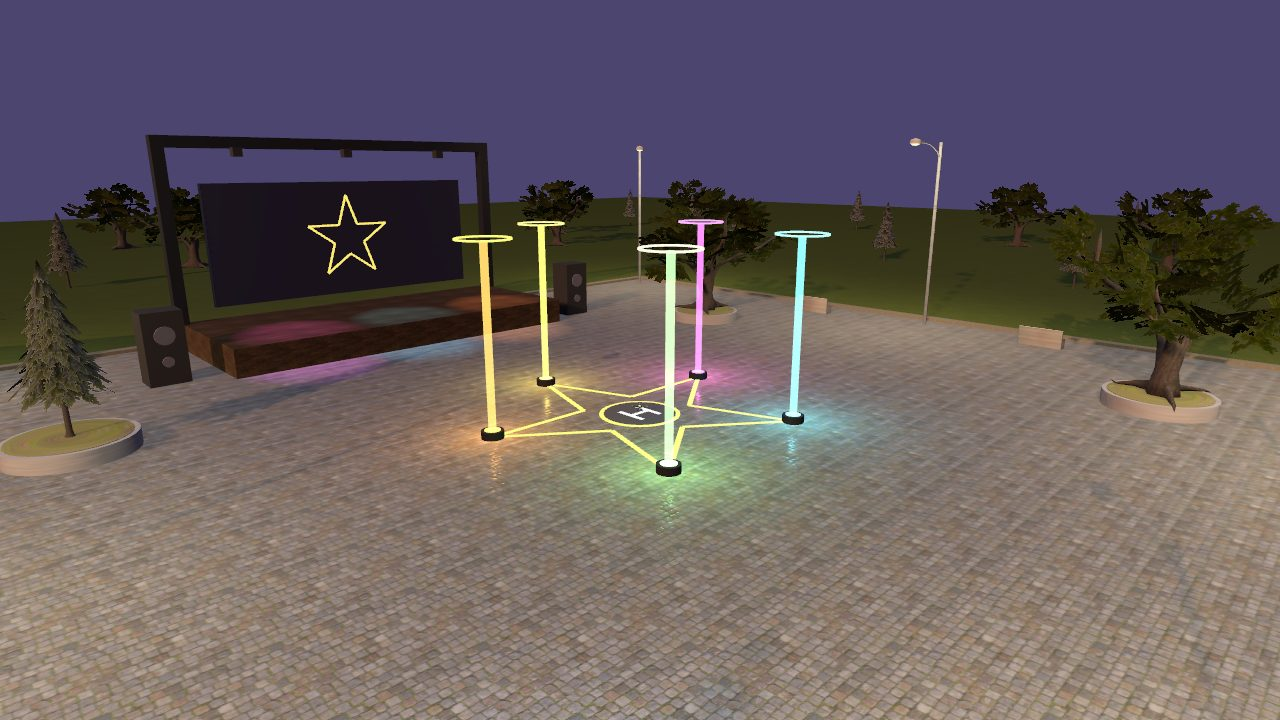
\includegraphics[width=\linewidth]{plaza_show_estrella}\\
    {\scriptsize \cmd{plaza\_show}: la estrella dorada y las 5 balizas con aros a 6 m}
    \column{0.33\textwidth}\centering
    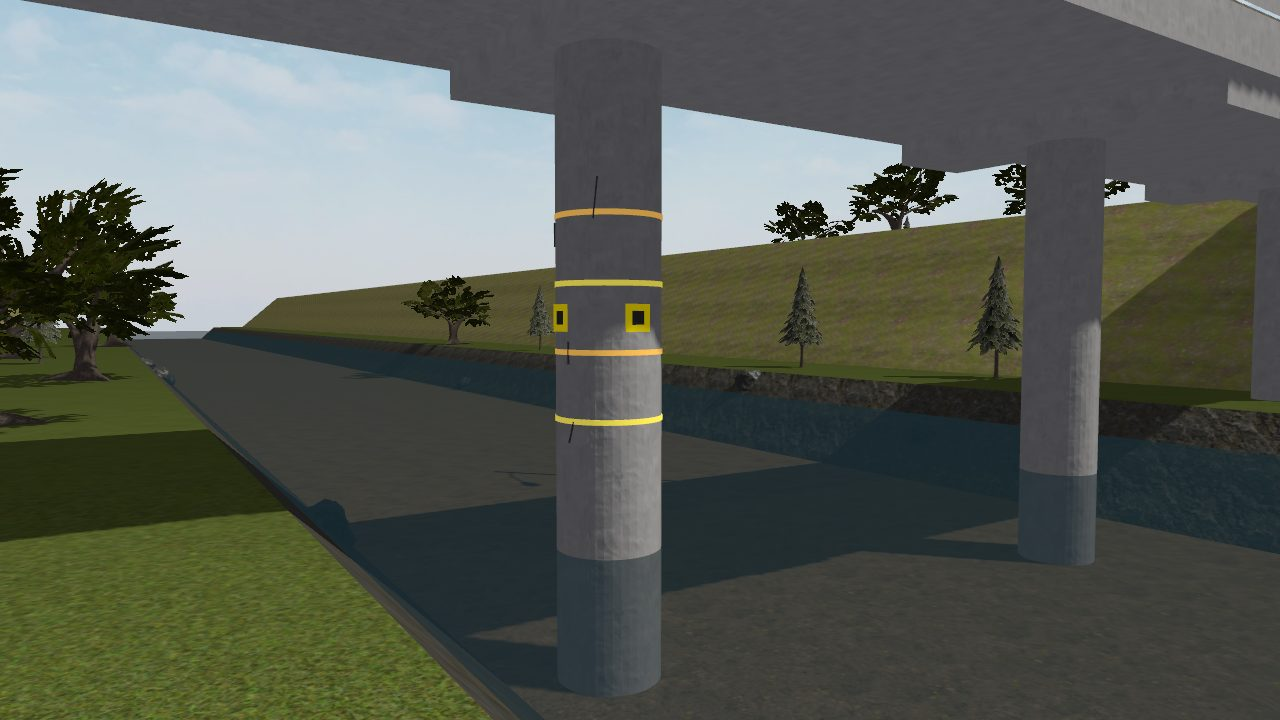
\includegraphics[width=\linewidth]{puente_rio_pilar}\\
    {\scriptsize \cmd{puente\_rio}: el pilar con bandas a 1, 2, 3 y 4 m}
    \column{0.33\textwidth}\centering
    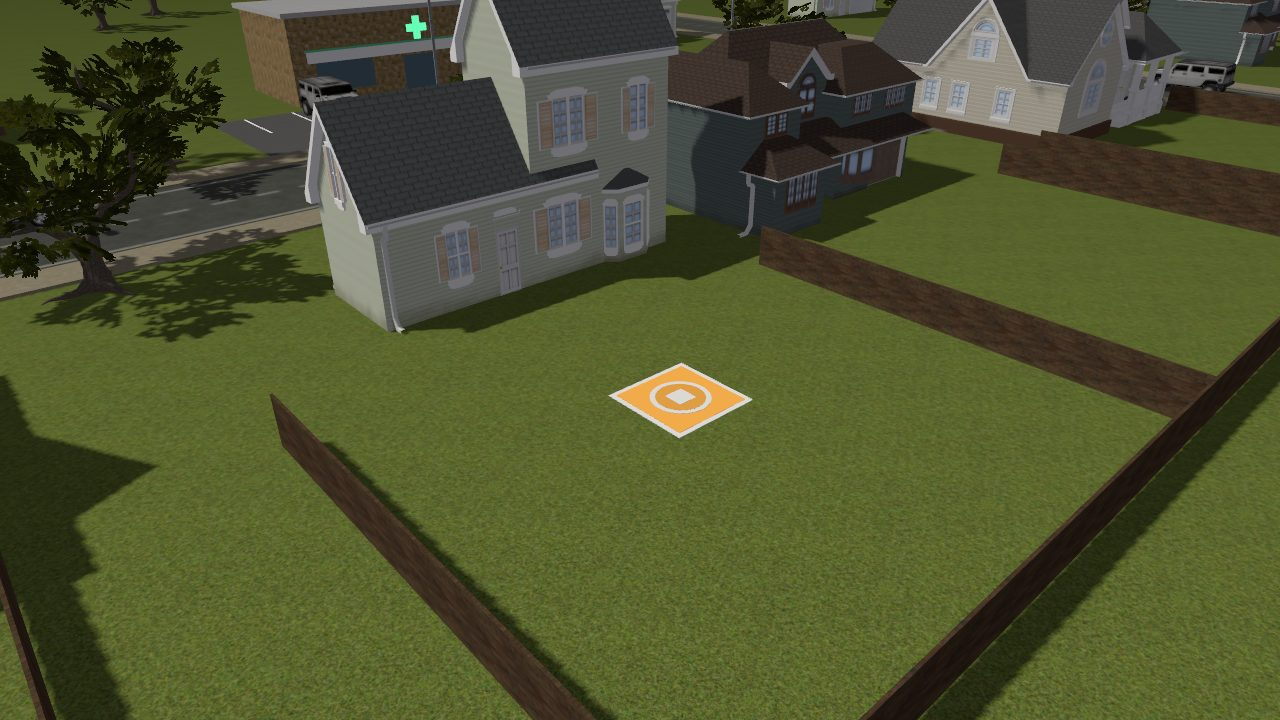
\includegraphics[width=\linewidth]{barrio_entrega_patio}\\
    {\scriptsize \cmd{barrio\_entrega}: la plataforma naranja en el patio, a 39.4 m}
  \end{columns}
\end{frame}

\begin{frame}{Los mundos (2/2)}
  \begin{columns}[t]
    \column{0.25\textwidth}\centering
    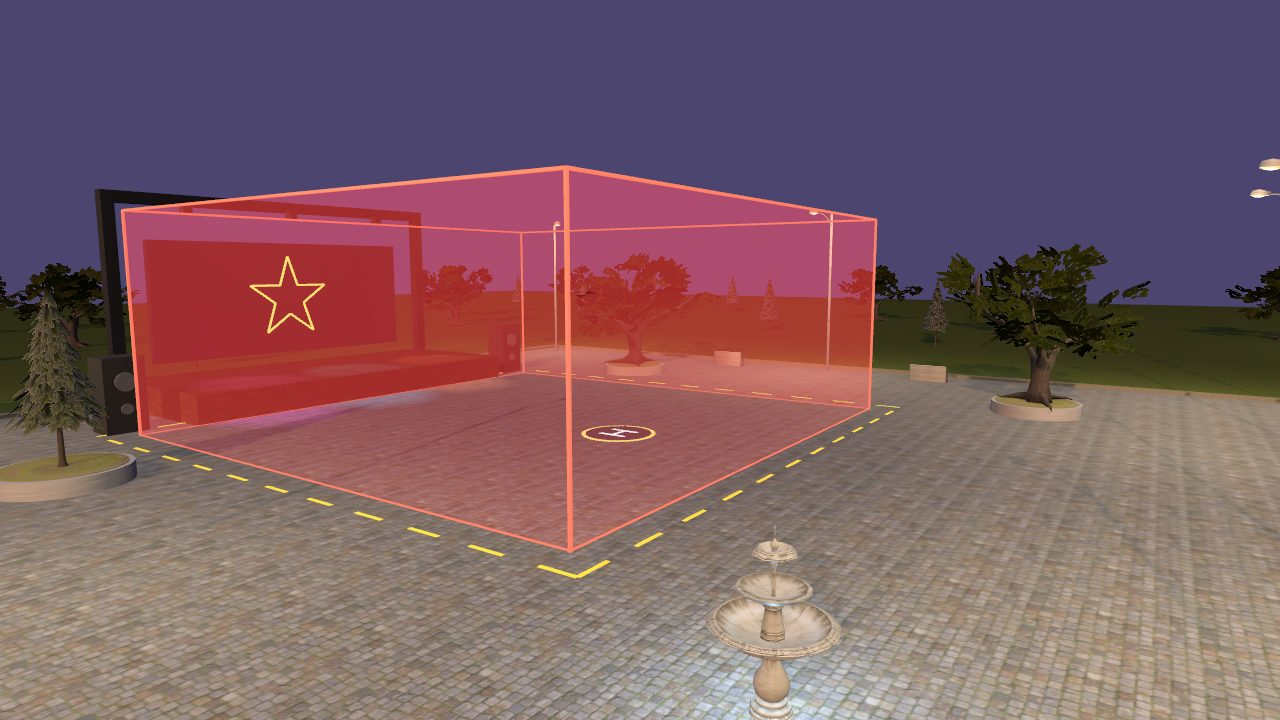
\includegraphics[width=\linewidth]{plaza_concierto}\\
    {\scriptsize \cmd{plaza\_concierto}: la geocerca roja}
    \column{0.25\textwidth}\centering
    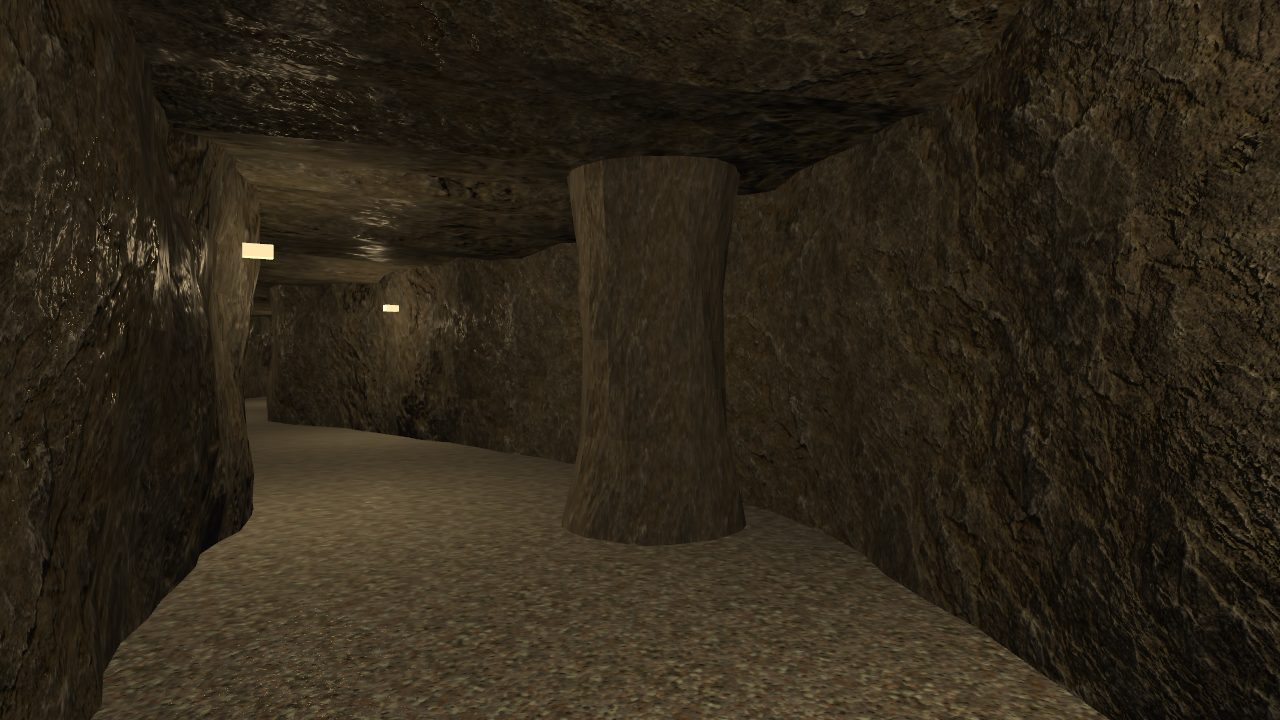
\includegraphics[width=\linewidth]{cueva_columna}\\
    {\scriptsize \cmd{cueva}: el túnel y la columna}
    \column{0.25\textwidth}\centering
    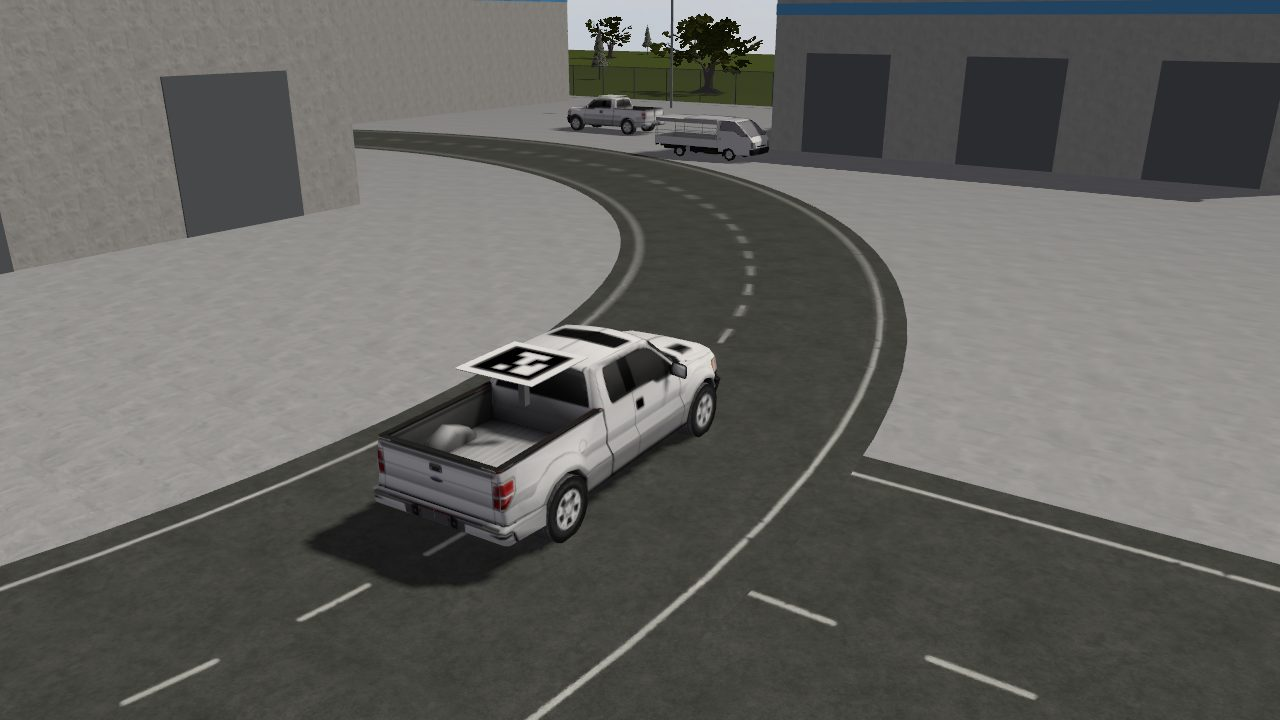
\includegraphics[width=\linewidth]{zona_bodegas_camioneta}\\
    {\scriptsize \cmd{zona\_bodegas}: la camioneta del ArUco 7}
    \column{0.25\textwidth}\centering
    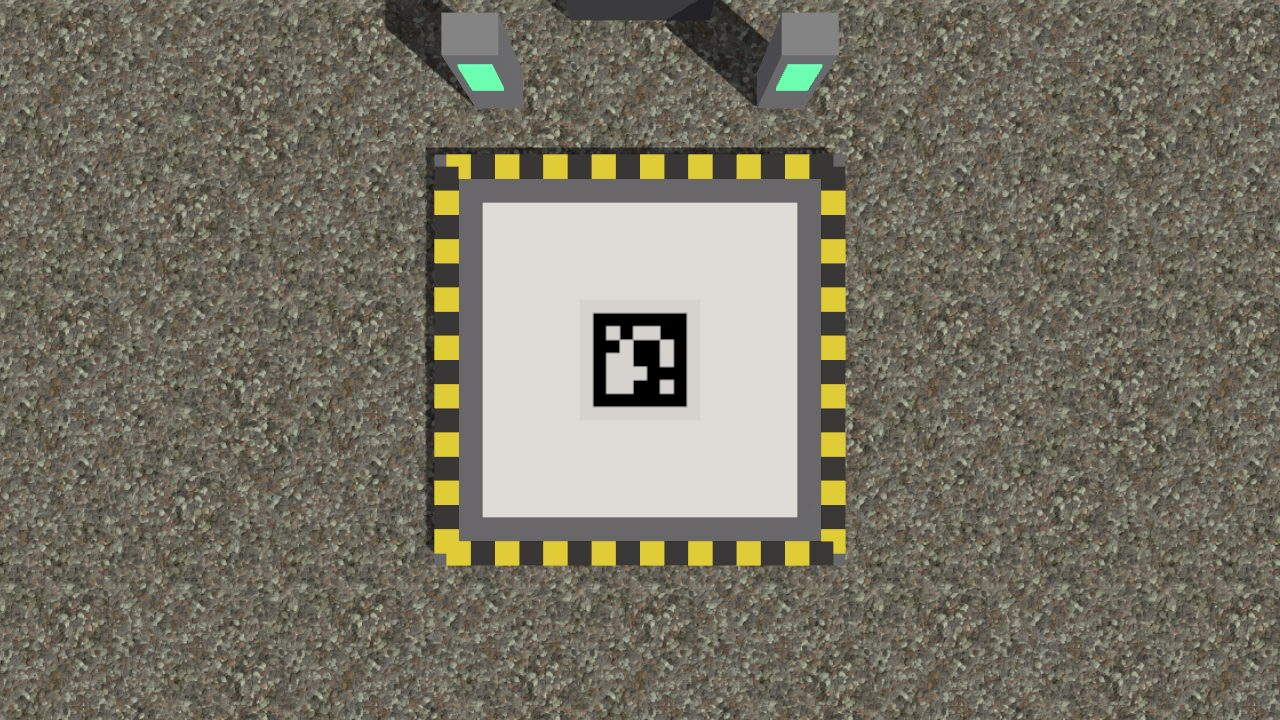
\includegraphics[width=\linewidth]{base_carga_estacion}\\
    {\scriptsize \cmd{base\_carga}: la estación con el ArUco 42}
  \end{columns}
\end{frame}

\begin{frame}{Cómo está hecho un reto}
  \begin{columns}[c]
    \column{0.52\textwidth}\small
    Cada misión es \textbf{un nodo que ya funciona}:
    \begin{itemize}
      \item La máquina de estados, los parámetros, el log y la medición del
        resultado \textbf{ya están hechos}.
      \item Lo que pide el reto está marcado con \cmd{// TODO} y pistas.
      \item Mientras no lo resuelvas, el nodo vuela de forma \textbf{segura}:
        despega, avisa qué falta, regresa y aterriza.
      \item Al final, el propio nodo te dice \textbf{``Misión cumplida''} o
        \textbf{``Misión NO cumplida''}.
    \end{itemize}
    \column{0.45\textwidth}
    \begin{terminal}{ros2 run x500\_retos estrella\_show}
OFFBOARD activo, subiendo a 6.0 m\\
vertices() regresó una lista vacía:\\
\ \ falta el TODO. Aterrizando\\
Aterrizado. Qué tan cerca pasó...\\
Misión NO cumplida
    \end{terminal}
  \end{columns}
\end{frame}

\begin{frame}{Qué se entrega por misión}
  \begin{enumerate}
    \item El nodo resuelto (los \cmd{TODO}), compilando \textbf{sin warnings}.
    \item Una corrida donde el nodo diga \textbf{``Misión cumplida''} (tres corridas seguidas para la rúbrica).
    \item Un README de 5 líneas: qué hace, cómo se corre, qué parámetros tiene.
    \item Un video corto de Gazebo + QGroundControl.
  \end{enumerate}
  \vspace{0.5em}
  \begin{idea}
    \textbf{Regla de oro:} nada de números mágicos. Alturas, radios, velocidades y
    tiempos van como parámetros (\cmd{--ros-args -p radio:=4.0}), igual que en
    \cmd{orbit\_mission}.
  \end{idea}
\end{frame}

\begin{frame}{Dónde vive cada cosa}
  \begin{columns}[c]
    \column{0.5\textwidth}
    \begin{tikzpicture}[every node/.style={font=\scriptsize\ttfamily,anchor=west}]
      \node at (0,0)    {src/x500\_retos/};
      \node at (0.3,-0.4) {include/x500\_retos/ \textrm{\color{gris}(px4\_link, aruco\_tools)}};
      \node at (0.3,-0.8) {src/ \textrm{\color{gris}(un .cpp por misión)}};
      \node at (0.3,-1.2) {msg/ \textrm{\color{gris}(Aruco, ArucoArray)}};
      \node at (0.3,-1.6) {launch/ \textrm{\color{gris}(cueva, caza, estacion)}};
      \node at (0.3,-2.0) {worlds/ \textrm{\color{gris}(los 7 mundos + spawn.yaml)}};
      \node at (0.3,-2.4) {models/ \textrm{\color{gris}(Fuel, texturas, x500\_cam\_abajo)}};
      \node at (0.3,-2.8) {tools/ \textrm{\color{gris}(build\_worlds, make\_aruco, render)}};
      \node at (0.3,-3.2) {docs/ \textrm{\color{gris}(capturas y esta presentación)}};
    \end{tikzpicture}
    \column{0.48\textwidth}\small
    \begin{itemize}
      \item \cmd{src/}: \textbf{aquí trabajan}.
      \item \cmd{include/}: lo que comparten todas las misiones; léanlo, no hace falta cambiarlo.
      \item \cmd{worlds/} se \textbf{genera} con \cmd{tools/build\_worlds.py}: cambios a mano se pierden.
      \item \cmd{CREDITS.md}: licencias de los modelos y texturas.
    \end{itemize}
  \end{columns}
\end{frame}

\begin{frame}{De dónde viene cada misión}
  \centering
  \begin{tikzpicture}[x=1cm,y=0.75cm,every node/.style={font=\scriptsize}]
    \tikzset{ex/.style={draw=gris,fill=gray!10,rounded corners,minimum width=2.5cm,minimum height=0.5cm},
             mi/.style={draw=azul,fill=azulclaro,rounded corners,minimum width=2.6cm,minimum height=0.5cm}}
    \node[ex] (sq) at (0,4) {square\_mission};
    \node[ex] (or) at (0,3) {orbit\_mission};
    \node[ex] (f8) at (0,2) {figure\_eight};
    \node[ex] (go) at (0,1) {goto\_mission};
    \node[ex] (rh) at (0,0) {return\_home / set\_home};
    \node[ex] (fm) at (0,-1) {flight\_mode\_monitor};
    \node[ex] (vc) at (0,-2) {velocity\_control};
    \node[ex] (bm) at (0,-3) {battery\_monitor};
    \node[mi] (m1) at (6,4) {1 estrella\_show};
    \node[mi] (m2) at (6,2.5) {2 inspeccion\_pilar};
    \node[mi] (m3) at (6,1) {3 entrega\_domicilio};
    \node[mi] (m4) at (6,-0.4) {4 guardian\_geocerca};
    \node[mi] (m5) at (6,-1.65) {5 cruzar\_cueva};
    \node[mi] (m6) at (6,-2.75) {6 caza\_objetivo};
    \node[mi] (m7) at (6,-3.85) {7 estacion\_carga};
    \draw[-{Stealth},gris] (sq) -- (m1); \draw[-{Stealth},gris] (or) -- (m1);
    \draw[-{Stealth},gris] (or) -- (m2); \draw[-{Stealth},gris] (f8) -- (m2);
    \draw[-{Stealth},gris] (go) -- (m3); \draw[-{Stealth},gris] (rh) -- (m3);
    \draw[-{Stealth},gris] (fm) -- (m4); \draw[-{Stealth},gris] (rh) -- (m4);
    \draw[-{Stealth},gris] (vc) -- (m5); \draw[-{Stealth},gris] (f8) -- (m6);
    \draw[-{Stealth},gris] (sq) -- (m7); \draw[-{Stealth},gris] (bm) -- (m7);
  \end{tikzpicture}
\end{frame}

% =============================================================================
\section{Preparar y correr}
% =============================================================================

\begin{frame}[fragile]{Compilar el workspace}
  \begin{lstlisting}[style=bash,caption={Una vez, y cada que cambie algo en src/}]
cd /data/vespo_ws
vespo build                 # colcon build de todo el workspace
source install/setup.bash   # en cada terminal nueva (vespo up lo hace solo)
  \end{lstlisting}
  \vspace{0.3em}
  \small
  \begin{itemize}
    \item \cmd{x500\_retos} instala los mundos, los modelos, los nodos, los launch y los mensajes.
    \item Al hacer \cmd{source}, un \emph{hook} agrega \cmd{share/x500\_retos/models} a
      \cmd{GZ\_SIM\_RESOURCE\_PATH}: así Gazebo encuentra \cmd{model://house\_1} y compañía.
    \item Si solo cambiaron su nodo: \cmd{colcon build --packages-select x500\_retos}.
  \end{itemize}
\end{frame}

\begin{frame}[fragile]{Levantar una misión: dos terminales}
  \begin{lstlisting}[style=bash,caption={Terminal 1: agente + PX4 SITL + Gazebo + QGroundControl}]
vespo up --sim --world plaza_show
  \end{lstlisting}
  \begin{lstlisting}[style=bash,caption={Terminal 2: tu nodo}]
ros2 run x500_retos estrella_show
ros2 run x500_retos estrella_show --ros-args -p points:=6 -p radius:=4.0
  \end{lstlisting}
  \begin{idea}
    \cmd{--world} elige el mundo; los de este paquete aparecen junto a los de PX4 en
    \cmd{vespo simulate --show}. Cada mundo trae un \cmd{spawn.yaml} que dice dónde
    aparece el dron.
  \end{idea}
\end{frame}

\begin{frame}{Mundo y modelo de cada misión}
  \centering\small
  \begin{tabular}{llll}
    \toprule
    Misión & \cmd{--world} & \cmd{--custom} & Cómo se corre \\
    \midrule
    1 & \cmd{plaza\_show} & --- (\cmd{x500}) & \cmd{ros2 run x500\_retos estrella\_show} \\
    2 & \cmd{puente\_rio} & --- & \cmd{ros2 run x500\_retos inspeccion\_pilar} \\
    3 & \cmd{barrio\_entrega} & --- & \cmd{ros2 run x500\_retos entrega\_domicilio} \\
    4 & \cmd{plaza\_concierto} & --- & \cmd{guardian\_geocerca} + \cmd{vuelo\_prueba} \\
    5 & \cmd{cueva} & \cmd{x500\_lidar\_2d} & \cmd{ros2 launch x500\_retos cueva.launch.py} \\
    6 & \cmd{zona\_bodegas} & \cmd{x500\_cam\_abajo} & \cmd{ros2 launch x500\_retos caza.launch.py} \\
    7 & \cmd{base\_carga} & \cmd{x500\_cam\_abajo} & \cmd{ros2 launch x500\_retos estacion.launch.py} \\
    \bottomrule
  \end{tabular}
  \vspace{0.6em}

  \footnotesize Ej.: \cmd{vespo up --sim --world cueva --custom x500\_lidar\_2d}
\end{frame}

\begin{frame}{Los tres modelos}
  \begin{columns}[t]
    \column{0.32\textwidth}
    \begin{idea}[title={\small\bfseries x500},coltitle=black,colbacktitle=azulclaro]
      \small El de siempre. Misiones 1--4.
    \end{idea}
    \column{0.32\textwidth}
    \begin{idea}[title={\small\bfseries x500\_lidar\_2d},coltitle=black,colbacktitle=azulclaro]
      \small De PX4: lidar 2D arriba, 1080 rayos en 270°, hasta 30 m, 30 Hz. Misión 5.
    \end{idea}
    \column{0.32\textwidth}
    \begin{idea}[title={\small\bfseries x500\_cam\_abajo},coltitle=black,colbacktitle=azulclaro]
      \small \textbf{Nuestro}: cámara hacia abajo de 960\,$\times$\,720 a 15 Hz. Misiones 6 y 7.
    \end{idea}
  \end{columns}
  \vspace{0.6em}
  \begin{ojo}
    \small No usen \cmd{x500\_mono\_cam\_down} de PX4 para el Nivel 3: su cámara es de
    1280\,$\times$\,960 a 30 Hz (\textasciitilde110 MB/s). Pasada a ROS, en una laptop de 16 GB nos
    llenó la RAM y trabó la computadora. Detalles en la sección de los mundos.
  \end{ojo}
\end{frame}

\begin{frame}{QGroundControl tiene que estar abierto}
  \begin{columns}[c]
    \column{0.55\textwidth}\small
    PX4 trae \cmd{NAV\_DLL\_ACT = 2}: si no hay estación de tierra, \textbf{no deja armar}.
    \begin{itemize}
      \item \cmd{vespo up --sim} ya abre QGC: no hay que hacer nada.
      \item Si corres \cmd{vespo simulate} solo, abre QGC con \cmd{vespo qgc}.
      \item Los nodos de offboard reintentan armar cada segundo: en cuanto QGC se conecta, arrancan.
    \end{itemize}
    \column{0.42\textwidth}
    \begin{terminal}{consola de PX4 (pxh>)}
WARN Preflight Fail:\\
\ \ No connection to the GCS\\
WARN Arming denied: Resolve\\
\ \ system health failures first
    \end{terminal}
  \end{columns}
\end{frame}

\begin{frame}[fragile]{Parámetros sin recompilar}
  \small Todo lo que es un número de la misión se declara como parámetro de ROS 2:
  \begin{lstlisting}[style=cpp,caption={Así se declaran (estrella\_show)}]
points_ = declare_parameter("points", 5);              // picos de la estrella
radius_ = declare_parameter("radius", 5.0);            // m, del centro a un pico
altitude_ = declare_parameter("altitude", 6.0);        // m sobre el despegue
  \end{lstlisting}
  \begin{lstlisting}[style=bash,caption={Y así se cambian}]
ros2 run x500_retos estrella_show --ros-args -p points:=4 -p inner_ratio:=0.0
ros2 param list /estrella_show          # con el nodo corriendo
  \end{lstlisting}
  \footnotesize El tipo sale del valor por defecto: \cmd{5} es entero, \cmd{5.0} es double.
  Pasar \cmd{points:=4.0} a un entero da error.
\end{frame}

\begin{frame}[fragile]{Ver qué está pasando}
  \begin{lstlisting}[style=bash,caption={Herramientas que conviene tener a la mano}]
ros2 topic list | grep fmu                     # lo que publica PX4
ros2 topic echo /fmu/out/vehicle_local_position_v1 --field z
ros2 topic hz /x500/scan                       # ¿llega el lidar?
ros2 run rqt_image_view rqt_image_view /x500/aruco/debug   # lo que ve el detector
gz topic -l | grep imager                      # topics de Gazebo (no de ROS)
vespo simulate --show                          # modelos y mundos disponibles
  \end{lstlisting}
  \begin{idea}
    \small ROS 2 y Gazebo tienen topics \textbf{distintos}. El lidar y la cámara publican en
    Gazebo; el \emph{launch} de cada misión levanta \cmd{ros\_gz\_bridge} para pasarlos a ROS.
  \end{idea}
\end{frame}

\begin{frame}{La computadora}
  \begin{itemize}
    \item \textbf{Con cargador}: Gazebo + PX4 + la GPU piden más de lo que da la batería
      de una laptop gamer en picos; sin cargador se nos apagó de golpe varias veces.
    \item \textbf{RAM}: una sesión normal usa \textasciitilde1--2 GB. Si Gazebo crece sin parar
      (\cmd{top}, columna RES de \cmd{ruby}), algo está acumulando imágenes: ciérrenlo.
    \item \textbf{Tiempo real}: el factor (RTF) de Gazebo debe estar cerca de 1.0
      (\cmd{gz topic -e -t /world/<mundo>/stats -n 1}). Todos los mundos corren a 1.0
      en una RTX 4060 laptop.
  \end{itemize}
\end{frame}

% =============================================================================
\section{Marcos de referencia}
% =============================================================================

\begin{frame}{Dos maneras de decir ``dónde''}
  \begin{columns}[c]
    \column{0.48\textwidth}\centering
    \textbf{Gazebo: ENU}\\[0.3em]
    \begin{tikzpicture}[scale=1.1]
      \draw[-{Stealth},thick,rojo] (0,0) -- (1.8,0) node[right,font=\scriptsize] {x = Este};
      \draw[-{Stealth},thick,verde] (0,0) -- (0,1.8) node[above,font=\scriptsize] {y = Norte};
      \draw[-{Stealth},thick,azul] (0,0) -- (-0.9,-0.7) node[below left,font=\scriptsize] {z = Arriba (hacia ti)};
      \fill (0,0) circle (1.5pt);
    \end{tikzpicture}\\
    \scriptsize Origen: el del mundo (lo decide quien hace el mundo).
    \column{0.48\textwidth}\centering
    \textbf{PX4: NED}\\[0.3em]
    \begin{tikzpicture}[scale=1.1]
      \draw[-{Stealth},thick,verde] (0,0) -- (0,1.8) node[above,font=\scriptsize] {x = Norte};
      \draw[-{Stealth},thick,rojo] (0,0) -- (1.8,0) node[right,font=\scriptsize] {y = Este};
      \draw[-{Stealth},thick,azul] (0,0) -- (0.9,-0.7) node[below right,font=\scriptsize] {z = Abajo};
      \fill (0,0) circle (1.5pt);
    \end{tikzpicture}\\
    \scriptsize Origen: \textbf{donde arrancó PX4}, no donde está el dron.
  \end{columns}
  \vspace{0.5em}
  \begin{idea}
    \small En NED \textbf{5 m arriba es $z = -5$}. Todas las alturas que mandamos a PX4 llevan signo menos.
  \end{idea}
\end{frame}

\begin{frame}{La convención de todos nuestros mundos}
  \begin{columns}[c]
    \column{0.5\textwidth}\small
    \begin{itemize}
      \item El dron aparece en \textbf{(0, 0) de Gazebo}, mirando al \textbf{norte}
        (\cmd{yaw\_deg: 90} en \cmd{spawn.yaml}).
      \item Así el origen de PX4 coincide con el del mundo y el heading arranca en 0.
      \item Pasar de uno a otro es solo cambiar el orden:
    \end{itemize}
    \[
      \begin{aligned}
        x_{\text{PX4}} &= y_{\text{Gazebo}} &&\text{(norte)}\\
        y_{\text{PX4}} &= x_{\text{Gazebo}} &&\text{(este)}\\
        z_{\text{PX4}} &= -z_{\text{Gazebo}} &&\text{(abajo)}
      \end{aligned}
    \]
    \column{0.47\textwidth}
    \begin{tikzpicture}[scale=0.8]
      \draw[gray!40,step=1] (-1,-1) grid (4,4);
      \draw[-{Stealth},thick,rojo] (0,0) -- (4.3,0) node[right,font=\tiny] {E (x Gz, y PX4)};
      \draw[-{Stealth},thick,verde] (0,0) -- (0,4.3) node[above,font=\tiny] {N (y Gz, x PX4)};
      \node[draw,circle,fill=azulclaro,inner sep=1pt,font=\tiny] at (0,0) {H};
      \fill[naranja] (3,2) circle (3pt) node[right,font=\tiny,black] {Gz (3, 2) = NED (2, 3)};
      \draw[-{Stealth},thick] (0,0.25) -- (0,0.8);
      \node[font=\tiny,left] at (0,0.6) {nariz};
    \end{tikzpicture}
  \end{columns}
\end{frame}

\begin{frame}{Ejemplo: el pilar del puente}
  \begin{columns}[c]
    \column{0.45\textwidth}
    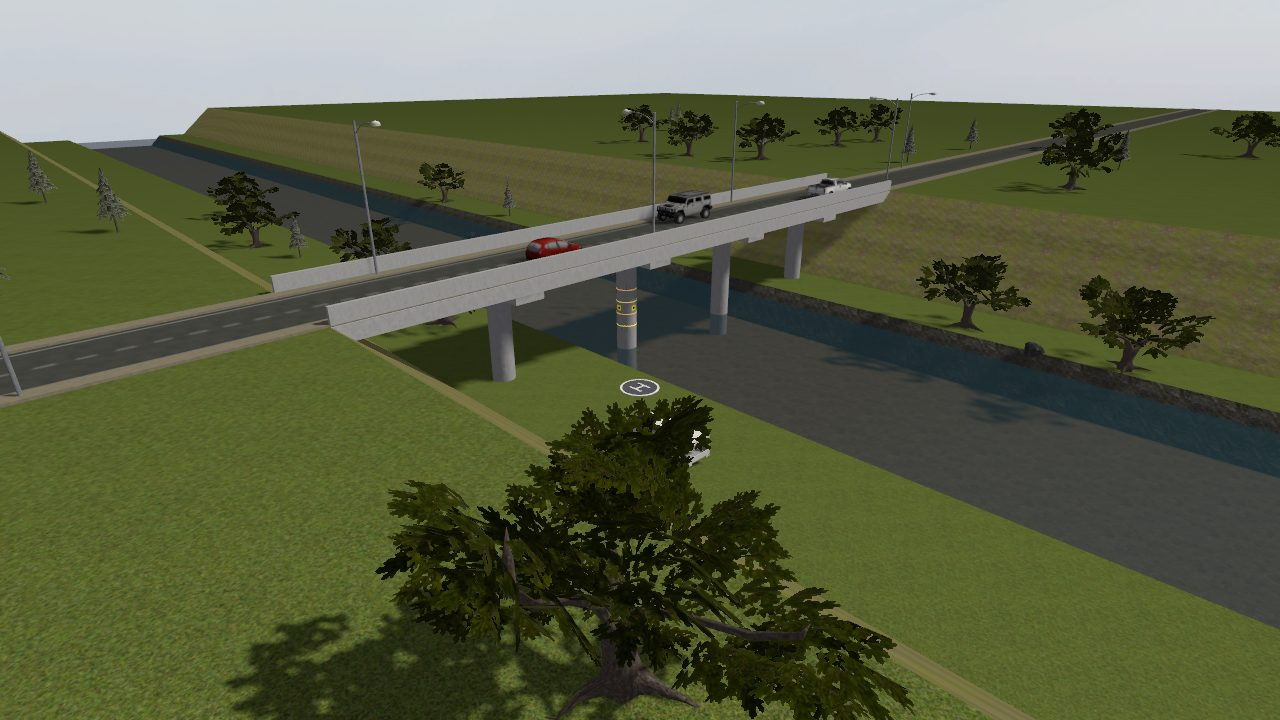
\includegraphics[width=\linewidth]{puente_rio}
    \column{0.52\textwidth}\small
    En \cmd{tools/build\_worlds.py} el pilar está en Gazebo \textbf{(6.5, 8.0)}.
    \begin{itemize}
      \item NED norte $= y_{Gz} = 8.0$ m
      \item NED este $= x_{Gz} = 6.5$ m
    \end{itemize}
    Por eso \cmd{inspeccion\_pilar} trae
    \cmd{center\_north = 8.0} y \cmd{center\_east = 6.5}.
    \vspace{0.4em}
    \begin{ojo}
      \small Si cambian de mundo o mueven el spawn, el origen de PX4 cambia y \textbf{todas}
      las coordenadas de la misión se recorren.
    \end{ojo}
  \end{columns}
\end{frame}

\begin{frame}{El marco del cuerpo: FRD}
  \begin{columns}[c]
    \column{0.45\textwidth}\centering
    \begin{tikzpicture}[scale=1.2]
      \draw[thick,fill=gray!20] (-0.5,-0.5) rectangle (0.5,0.5);
      \foreach \x/\y in {-0.7/0.7,0.7/0.7,-0.7/-0.7,0.7/-0.7} {\draw[gray] (\x,\y) circle (0.3);}
      \draw[-{Stealth},thick,verde] (0,0) -- (0,1.4) node[above,font=\scriptsize] {x: Frente};
      \draw[-{Stealth},thick,rojo] (0,0) -- (1.4,0) node[right,font=\scriptsize] {y: Derecha};
      \node[font=\scriptsize] at (0.1,-1.25) {z: Abajo (entrando)};
      \draw[-{Stealth},azul,thick] (0.55,1.0) arc (60:20:0.9) node[right,font=\scriptsize] {yaw $+$};
    \end{tikzpicture}
    \column{0.52\textwidth}\small
    \begin{itemize}
      \item PX4 describe el dron en \textbf{FRD}: x al frente, y a la derecha, z abajo.
      \item El \textbf{heading} (yaw) es el ángulo del frente medido desde el norte,
        \textbf{positivo hacia el este} (en sentido horario visto desde arriba).
      \item \cmd{vehicle\_local\_position.heading}: el yaw actual, en radianes $[-\pi, \pi]$.
      \item \cmd{vehicle\_attitude.q}: la actitud completa (roll, pitch y yaw) como cuaternión.
    \end{itemize}
  \end{columns}
\end{frame}

\begin{frame}{Del cuerpo a NED: rotar por el heading}
  \small Si el dron va nivelado, una velocidad ``adelante / derecha'' se pasa a NED así:
  \[
    \begin{pmatrix} v_N \\ v_E \end{pmatrix} =
    \begin{pmatrix} \cos\psi & -\sin\psi \\ \sin\psi & \cos\psi \end{pmatrix}
    \begin{pmatrix} v_{\text{adelante}} \\ v_{\text{derecha}} \end{pmatrix}
  \]
  \begin{columns}[c]
    \column{0.5\textwidth}
    \begin{itemize}
      \item $\psi = 0$ (mirando al norte): adelante = norte, derecha = este.
      \item $\psi = 90^\circ$ (mirando al este): adelante = este, derecha = sur.
    \end{itemize}
    \column{0.45\textwidth}
    \begin{ojo}
      \small El lidar y ROS usan \textbf{FLU} (y a la \emph{izquierda}, ángulos positivos
      a la izquierda). PX4 usa FRD. En la cueva hay que voltear signos: lo vemos ahí.
    \end{ojo}
  \end{columns}
\end{frame}

\begin{frame}{Ángulos: siempre envolver a $[-\pi, \pi]$}
  \small Restar ángulos ``a lo bruto'' falla cerca de $\pm180^\circ$:
  \[ 179° - (-179°) = 358° \quad\text{pero en realidad son } 2°. \]
  En \cmd{px4\_link.hpp}:
  \[ \text{wrap\_pi}(a) = \operatorname{atan2}(\sin a, \cos a) \in [-\pi, \pi] \]
  \begin{idea}
    \small Úsenlo cada vez que comparen dos yaws (error de apuntado en el pilar, giro hacia un hueco, etc.).
  \end{idea}
\end{frame}

\begin{frame}{De metros a GPS (y de vuelta)}
  \small Los comandos de PX4 (\cmd{DO\_REPOSITION}, \cmd{NAV\_TAKEOFF}, \cmd{DO\_SET\_HOME}) piden
  \textbf{latitud y longitud}. Para unos cuantos km basta la Tierra plana ($R = 6\,371\,000$ m):
  \[
    \text{lat} = \text{lat}_0 + \frac{\Delta N}{R}\cdot\frac{180}{\pi}
    \qquad
    \text{lon} = \text{lon}_0 + \frac{\Delta E}{R\cos(\text{lat}_0)}\cdot\frac{180}{\pi}
  \]
  \begin{itemize}
    \item Los meridianos se juntan hacia los polos: por eso el $\cos(\text{lat})$ en la longitud.
    \item Ya están hechas: \cmd{x500::gps\_offset()} y \cmd{x500::gps\_distance()}.
    \item \cmd{lat} y \cmd{lon} van en \cmd{double} (param5 y param6 del comando): en
      \cmd{float} se pierde \textasciitilde1 m.
  \end{itemize}
\end{frame}

\begin{frame}{¿Dónde está nuestro mundo en el planeta?}
  \small Todos los mundos usan la ubicación de los mundos de PX4 (Zúrich):
  \[ \text{lat}_0 = 47.397971^\circ \qquad \text{lon}_0 = 8.546164^\circ \]
  \begin{ojo}
    \small El \cmd{<magnetic\_field>} del mundo corresponde a ese lugar. Si cambian la ubicación sin
    cambiar el campo magnético, el chequeo de brújula de PX4 falla
    (\emph{``strong magnetic interference''}).
  \end{ojo}
  \vspace{0.3em}
  Ejemplo: la plataforma del barrio está 36 m al norte y 16 m al este de la farmacia
  $\Rightarrow$ lat 47.3982949, lon 8.5463757.
\end{frame}

% =============================================================================
\section{px4\_link.hpp: lo que comparten todas}
% =============================================================================

\begin{frame}{Por qué una clase común}
  \begin{columns}[c]
    \column{0.5\textwidth}\small
    En \cmd{px4\_examples} cada nodo repetía \textasciitilde80 líneas:
    suscripciones, publishers, \cmd{send\_command()}, \cmd{now\_us()}\ldots
    \vspace{0.4em}

    Aquí eso vive en \cmd{x500::Px4Link} y cada misión se queda solo con
    \textbf{su máquina de estados}.
    \vspace{0.4em}
    \begin{idea}
      \small Si PX4 cambia la versión de un mensaje (\cmd{vehicle\_status\_v1}\ldots),
      se corrige en un solo archivo.
    \end{idea}
    \column{0.47\textwidth}
    \begin{tikzpicture}[every node/.style={font=\scriptsize}]
      \node[draw=azul,fill=azulclaro,rounded corners,minimum width=2.4cm,minimum height=1.6cm] (l) {Px4Link};
      \node[draw,rounded corners,left=1.2cm of l,minimum width=1.4cm] (p) {PX4};
      \node[draw=azul,rounded corners,above=0.7cm of l,minimum width=2.4cm] (n) {tu misión};
      \draw[-{Stealth}] ([yshift=0.4cm]p.east) -- node[above,font=\tiny] {/fmu/out} ([yshift=0.4cm]l.west);
      \draw[{Stealth}-] ([yshift=-0.4cm]p.east) -- node[below,font=\tiny] {/fmu/in} ([yshift=-0.4cm]l.west);
      \draw[{Stealth}-{Stealth}] (n) -- (l);
    \end{tikzpicture}
  \end{columns}
\end{frame}

\begin{frame}[fragile]{Uso}
  \begin{lstlisting}[style=cpp,caption={Dentro de cualquier rclcpp::Node}]
#include "x500_retos/px4_link.hpp"

class MiMision : public rclcpp::Node {
  x500::Px4Link px4_{this};         // crea suscripciones y publishers

  void loop() {
    const auto & l = px4_.local();  // posición NED (m), velocidad, heading
    if (px4_.armed() && px4_.in_offboard()) { ... }
    px4_.offboard(setpoint);        // heartbeat + setpoint, CADA ciclo
    px4_.command(VehicleCommand::VEHICLE_CMD_NAV_LAND);
  }
};
  \end{lstlisting}
\end{frame}

\begin{frame}{Lo que lee de PX4}
  \centering\small
  \begin{tabular}{lll}
    \toprule
    Método & Topic & Para qué \\
    \midrule
    \cmd{status()} & \cmd{/fmu/out/vehicle\_status\_v1} & armado, modo (nav\_state) \\
    \cmd{local()} & \cmd{/fmu/out/vehicle\_local\_position\_v1} & x, y, z, vx, vy, vz, heading \\
    \cmd{global()} & \cmd{/fmu/out/vehicle\_global\_position} & lat, lon, alt (AMSL) \\
    \cmd{home()} & \cmd{/fmu/out/home\_position\_v1} & dónde está ``casa'' \\
    \cmd{attitude()} & \cmd{/fmu/out/vehicle\_attitude} & cuaternión q = \{w, x, y, z\} \\
    \bottomrule
  \end{tabular}
  \vspace{0.6em}

  \raggedright Y atajos: \cmd{armed()}, \cmd{in\_offboard()}, \cmd{in\_hold()}, \cmd{local\_ready()},
  \cmd{gps\_ready()}, \cmd{distance\_to(p)}.
  \vspace{0.3em}
  \begin{idea}
    \small También escucha \cmd{vehicle\_command\_ack} y avisa con un \cmd{WARN} cuando PX4
    \textbf{rechaza} un comando (una vez por cada respuesta distinta).
  \end{idea}
\end{frame}

\begin{frame}[fragile]{El setpoint de offboard}
  \begin{lstlisting}[style=cpp,caption={x500::Setpoint: lo que se deja en NaN, PX4 no lo usa}]
struct Setpoint {
  std::array<float, 3> position{kNaN, kNaN, kNaN};      // m, NED
  std::array<float, 3> velocity{kNaN, kNaN, kNaN};      // m/s
  std::array<float, 3> acceleration{kNaN, kNaN, kNaN};  // m/s^2
  float yaw = kNaN;        // rad, 0 = norte, + hacia el este
  float yawspeed = kNaN;   // rad/s, feedforward de giro
};
  \end{lstlisting}
  \small \cmd{offboard(sp)} publica dos cosas, cada vez:
  \begin{enumerate}
    \item \cmd{OffboardControlMode}: qué campos traen valor (el \emph{heartbeat}).
    \item \cmd{TrajectorySetpoint}: los valores.
  \end{enumerate}
\end{frame}

\begin{frame}{Setpoints mixtos}
  \small Basta un eje con valor para que ese tipo cuente. Así se combinan:
  \vspace{0.3em}
  \centering
  \begin{tabular}{lll}
    \toprule
    position & velocity & Qué hace PX4 \\
    \midrule
    $\{N, E, Z\}$ & NaN & ir a ese punto \\
    $\{N, E, Z\}$ & $\{v_N, v_E, v_Z\}$ & ir al punto usando la velocidad como \emph{feedforward} \\
    $\{\text{NaN}, \text{NaN}, Z\}$ & $\{v_N, v_E, \text{NaN}\}$ & avanzar por velocidad a altura fija (cueva, vuelo\_prueba) \\
    $\{N, E, \text{NaN}\}$ & $\{\text{NaN}, \text{NaN}, v_Z\}$ & quedarse en $(N, E)$ bajando a $v_Z$ (aterrizaje de precisión) \\
    \bottomrule
  \end{tabular}
\end{frame}

\begin{frame}{Feedforward: no ir ``atrás'' del setpoint}
  \begin{columns}[c]
    \column{0.5\textwidth}
    \begin{tikzpicture}[scale=0.9]
      \draw[gray!50] (0,0) circle (1.6);
      \draw[-{Stealth},azul,thick] (1.6,0) arc (0:70:1.6);
      \fill[azul] (70:1.6) circle (2pt) node[above right,font=\tiny] {setpoint};
      \fill[rojo] (35:1.6) circle (2pt) node[right,font=\tiny] {dron (solo posición)};
      \fill[verde] (64:1.6) circle (2pt) node[left,font=\tiny,xshift=-2pt] {con feedforward};
    \end{tikzpicture}
    \column{0.48\textwidth}\small
    \begin{itemize}
      \item Con \textbf{solo posición}, PX4 corrige \emph{después} de ver el error: en una
        trayectoria que se mueve, siempre va atrás.
      \item Con la \textbf{velocidad} (y aceleración) de la trayectoria, ya sabe cómo moverse:
        el error queda casi en cero.
      \item Lo mismo con el yaw: \cmd{yawspeed} le dice qué tan rápido girar.
    \end{itemize}
  \end{columns}
\end{frame}

\begin{frame}{El heartbeat de offboard}
  \centering
  \begin{tikzpicture}[x=1.1cm]
    \draw[-{Stealth}] (0,0) -- (10.5,0) node[right,font=\scriptsize] {t};
    \foreach \x in {0.25,0.5,...,10} \draw[azul] (\x,0) -- (\x,0.3);
    \node[font=\tiny,azul,above] at (1.25,0.3) {setpoints a 20 Hz};
    \draw[-{Stealth},thick,naranja] (1,-0.9) -- (1,-0.05);
    \node[font=\tiny,below,align=center] at (1,-0.9) {$\approx$1 s: pedir\\OFFBOARD + armar};
    \draw[-{Stealth},thick,verde] (2.2,-0.9) -- (2.2,-0.05);
    \node[font=\tiny,below,align=center] at (2.6,-0.9) {PX4 entra\\a offboard};
    \draw[rojo,thick] (7.5,-0.1) -- (7.5,0.6);
    \node[font=\tiny,rojo,align=center] at (8.6,0.9) {el nodo se cae: \textgreater0.5 s sin\\heartbeat = failsafe};
  \end{tikzpicture}
  \vspace{0.6em}
  \begin{itemize}\small
    \item PX4 \textbf{no entra} a offboard si no está recibiendo setpoints ya.
    \item Mientras el nodo controla, hay que publicar \textbf{en cada ciclo} (todos usan un timer de 50 ms).
    \item Si se deja de publicar, PX4 entra en failsafe: eso también se prueba a propósito.
  \end{itemize}
\end{frame}

\begin{frame}{Comandos que usamos}
  \centering\scriptsize
  \begin{tabular}{lll}
    \toprule
    Comando & Parámetros & Atajo en Px4Link \\
    \midrule
    \cmd{DO\_SET\_MODE} & p1 = 1, p2 = 6 (OFFBOARD) & \cmd{request\_offboard\_and\_arm()} \\
    \cmd{DO\_SET\_MODE} & p1 = 1, p2 = 4, p3 = 3 (Hold) & \cmd{request\_hold()} \\
    \cmd{COMPONENT\_ARM\_DISARM} & p1 = 1 & \cmd{arm()} \\
    \cmd{NAV\_LAND} & --- & \cmd{land()} \\
    \cmd{NAV\_RETURN\_TO\_LAUNCH} & --- & \cmd{return\_home()} \\
    \cmd{NAV\_TAKEOFF} & p5, p6 = lat, lon; p7 = alt AMSL & \cmd{command(...)} \\
    \cmd{DO\_REPOSITION} & p1 = vel, p2 = 1, p5..p7 = lat, lon, alt & \cmd{command(...)} \\
    \cmd{DO\_SET\_HOME} & p1 = 0, p5..p7 = lat, lon, alt & \cmd{command(...)} \\
    \bottomrule
  \end{tabular}
  \vspace{0.5em}

  \raggedright\footnotesize \textbf{Hold antes de armar}: desde Land (como queda al aterrizar) PX4 no deja armar.
  Por eso \cmd{entrega\_domicilio} pasa por Hold antes de volver a despegar.
\end{frame}

\begin{frame}{El reloj de PX4, no el de la pared}
  \begin{columns}[c]
    \column{0.55\textwidth}\small
    PX4 SITL corre en \emph{lockstep} con Gazebo: si la simulación va lenta, PX4 también.
    Pero \cmd{now()} de ROS es el reloj de la pared.
    \vspace{0.3em}

    En una prueba el mundo del puente corría a \textbf{0.27$\times$}: la hélice ``avanzaba''
    casi 4 veces más rápido de lo que el dron podía seguir y el yaw se quedaba 40° atrás.
    \vspace{0.3em}
    \begin{idea}
      \small \cmd{px4\_.clock()}: el timestamp de la posición de PX4, en segundos. Úsenlo para
      todo lo que dependa del tiempo de la misión.
    \end{idea}
    \column{0.42\textwidth}
    \begin{tikzpicture}[x=0.55cm,y=0.5cm]
      \draw[-{Stealth}] (0,0) -- (7,0) node[right,font=\tiny] {pared (s)};
      \draw[-{Stealth}] (0,0) -- (0,5) node[above,font=\tiny] {simulación (s)};
      \draw[verde,thick] (0,0) -- (6,4.5) node[right,font=\tiny] {RTF 1.0};
      \draw[rojo,thick] (0,0) -- (6,1.6) node[right,font=\tiny] {RTF 0.27};
    \end{tikzpicture}
  \end{columns}
\end{frame}

% =============================================================================
\section{Máquinas de estados}
% =============================================================================

\begin{frame}{Todas las misiones tienen la misma forma}
  \centering
  \begin{tikzpicture}[node distance=0.45cm,
      st/.style={draw=azul,fill=azulclaro,rounded corners,font=\scriptsize,minimum height=0.6cm,minimum width=1.5cm}]
    \node[st] (w) {WARMUP};
    \node[st,right=of w] (t) {TAKEOFF};
    \node[st,right=of t,fill=yellow!20] (m) {\textbf{LA MISIÓN}};
    \node[st,right=of m] (l) {LANDING};
    \node[st,right=of l] (d) {DONE};
    \draw[-{Stealth}] (w) -- node[above,font=\tiny] {offboard} (t);
    \draw[-{Stealth}] (t) -- node[above,font=\tiny] {altura} (m);
    \draw[-{Stealth}] (m) -- node[above,font=\tiny] {land()} (l);
    \draw[-{Stealth}] (l) -- node[above,font=\tiny] {desarmó} (d);
    \draw[-{Stealth},rojo,dashed] (m.south) to[bend right=25] node[below,font=\tiny] {ya no está en offboard: abortar} (d.south);
  \end{tikzpicture}
  \vspace{0.7em}
  \begin{itemize}\small
    \item \textbf{WARMUP}: \textasciitilde1 s de setpoints, luego OFFBOARD + armar (reintentando cada segundo).
    \item \textbf{TAKEOFF}: subir sobre el despegue hasta la altura de la misión.
    \item \textbf{LA MISIÓN}: uno o varios estados propios (vértices, hélice, barrido\ldots).
    \item \textbf{LANDING}: PX4 aterriza y desarma solo; entonces se imprime el resultado.
    \item \textbf{DONE}: \cmd{rclcpp::shutdown()}, así \cmd{ros2 run} regresa a la terminal.
  \end{itemize}
\end{frame}

\begin{frame}[fragile]{En código: enum class + switch}
  \begin{lstlisting}[style=cpp,caption={El esqueleto (simplificado de estrella\_show)}]
enum class State { WARMUP, TAKEOFF, STAR, CENTER, LANDING, DONE };

void loop() {                       // timer de 50 ms
  switch (state_) {
    case State::WARMUP:
      px4_.offboard(hover(center));
      if (++counter_ % 20 == 0) px4_.request_offboard_and_arm();   // cada 1 s
      if (px4_.in_offboard()) state_ = State::TAKEOFF;
      return;
    case State::TAKEOFF: ...  break;
    case State::STAR:    ...  break;    // la misión
    case State::LANDING:
      if (!px4_.armed()) { report(); state_ = State::DONE; }
      return;
    case State::DONE: rclcpp::shutdown(); return;
  }
  if (state_ != State::LANDING && !px4_.in_offboard()) state_ = State::DONE;  // abortar
}
  \end{lstlisting}
\end{frame}

\begin{frame}{Reglas que siguen todos los nodos}
  \begin{enumerate}\small
    \item \textbf{Cada \cmd{case} termina en \cmd{break} o \cmd{return}}. Sin él, el código sigue en el case de abajo.
    \item \textbf{Una transición = un log}: \cmd{RCLCPP\_INFO} al cambiar de estado, para seguir la misión en la terminal.
    \item \textbf{Logs repetidos con throttle}: \cmd{RCLCPP\_INFO\_THROTTLE(..., 2000, ...)} como mucho cada 2 s.
    \item \textbf{Si alguien toma el control, el nodo suelta}: fuera de OFFBOARD deja de mandar setpoints
      (el piloto o el guardián manda).
    \item \textbf{El nodo se califica solo}: mide durante el vuelo y al aterrizar imprime OK / FALLÓ por criterio.
  \end{enumerate}
\end{frame}

\begin{frame}{Antes de programar: dibujar la máquina}
  \begin{columns}[c]
    \column{0.5\textwidth}\small
    La rúbrica pide \textbf{explicar la máquina de estados en voz alta}. Antes de escribir código:
    \begin{enumerate}
      \item Escribe los estados.
      \item Para cada uno: qué setpoint o comando manda.
      \item Para cada flecha: qué condición la dispara.
      \item ¿Qué pasa si algo falla en cada estado?
    \end{enumerate}
    \column{0.47\textwidth}
    \begin{idea}
      \small Una buena prueba: si alguien de otro equipo puede leer tu diagrama y adivinar qué
      va a hacer el dron, está bien.
    \end{idea}
  \end{columns}
\end{frame}

% =============================================================================
\section{Cómo están hechos los mundos}
% =============================================================================

\begin{frame}{Un mundo = un .sdf generado}
  \begin{columns}[c]
    \column{0.5\textwidth}
    \begin{tikzpicture}[node distance=0.5cm,every node/.style={font=\scriptsize}]
      \node[draw=azul,fill=azulclaro,rounded corners,minimum width=3.4cm] (b) {tools/build\_worlds.py};
      \node[draw,rounded corners,below left=0.6cm and -1.2cm of b,minimum width=2.2cm,align=center] (m) {models/x500\_mallas\\(.obj con UVs)};
      \node[draw,rounded corners,below right=0.6cm and -1.2cm of b,minimum width=2.2cm,align=center] (w) {worlds/<mundo>/\\<mundo>.sdf + spawn.yaml};
      \node[draw,rounded corners,below=1.9cm of b,minimum width=3.4cm,align=center] (f) {models/: Fuel + texturas\\(copiados, sin internet)};
      \draw[-{Stealth}] (b) -- (m); \draw[-{Stealth}] (b) -- (w);
      \draw[-{Stealth},dashed] (f) -- (w);
    \end{tikzpicture}
    \column{0.47\textwidth}\small
    \begin{itemize}
      \item \cmd{python3 tools/build\_worlds.py} reescribe \textbf{todos} los mundos.
      \item Cambiar un mundo = cambiar el script y regenerar. Cambios a mano en el
        \cmd{.sdf} se pierden.
      \item Luego \cmd{vespo build} para instalarlos.
    \end{itemize}
  \end{columns}
\end{frame}

\begin{frame}{Las piezas}
  \begin{columns}[t]
    \column{0.32\textwidth}
    \begin{idea}[title={\small\bfseries Modelos de Fuel},coltitle=black,colbacktitle=azulclaro]
      \scriptsize Casas, árboles, coches, postes, fuente, bancas, camión, rocas (OpenRobotics,
      CC0 / CC BY). Copiados en \cmd{models/}.
    \end{idea}
    \column{0.32\textwidth}
    \begin{idea}[title={\small\bfseries Texturas},coltitle=black,colbacktitle=azulclaro]
      \scriptsize De ambientCG (CC0): pasto, adoquín, concreto, calle, roca, madera, ladrillo, grava.
      Color + normal + rugosidad (PBR).
    \end{idea}
    \column{0.32\textwidth}
    \begin{idea}[title={\small\bfseries Lo propio},coltitle=black,colbacktitle=azulclaro]
      \scriptsize Piso, puente, farmacia, cueva, bodegas, balizas, geocerca, estación: cajas,
      cilindros y mallas que escribe el script.
    \end{idea}
  \end{columns}
  \vspace{0.5em}
  \small Licencias y lista completa en \cmd{CREDITS.md}.
\end{frame}

\begin{frame}{¿Por qué mallas y no un \texttt{<plane>}?}
  \begin{columns}[c]
    \column{0.5\textwidth}\small
    Un \cmd{<plane>} de Gazebo estira \textbf{una} imagen sobre todo su tamaño: una textura de
    pasto de 1 m sobre 260 m se ve borrosa.
    \vspace{0.3em}

    El script escribe mallas \cmd{.obj} cuyas coordenadas UV son \emph{metros / tamaño del mosaico}:
    la textura se repite cada 2--4 m.
    \column{0.47\textwidth}
    \begin{tikzpicture}[scale=0.55]
      \draw[fill=green!35] (0,0) rectangle (4,4);
      \node[font=\tiny] at (2,-0.4) {\texttt{<plane>}: 1 imagen};
      \begin{scope}[xshift=5cm]
        \foreach \i in {0,1,2,3} \foreach \j in {0,1,2,3} \draw[fill=green!25!yellow!30] (\i,\j) rectangle (\i+1,\j+1);
        \node[font=\tiny] at (2,-0.4) {malla: mosaico};
      \end{scope}
    \end{tikzpicture}
  \end{columns}
\end{frame}

\begin{frame}{Colisiones: siempre cajas}
  \small
  \begin{itemize}
    \item El motor de física de Gazebo (dartsim) no choca de forma confiable contra \textbf{mallas}.
    \item Por eso lo propio lleva \textbf{cajas y cilindros} como colisión, aunque se vea con malla:
      el puente, las paredes de la cueva (una caja cada \textasciitilde1 m), las bodegas, la cerca.
    \item Las paredes rojas de la geocerca y los haces de las balizas son \textbf{solo visuales}:
      el dron las atraviesa.
  \end{itemize}
  \begin{ojo}
    \small Si agregan un obstáculo, agreguen su \cmd{collision()} además del \cmd{visual()}.
    Si solo se ve, el dron lo atraviesa; si solo choca, el lidar o la cámara no lo ven.
  \end{ojo}
\end{frame}

\begin{frame}[fragile]{Agregar algo a un mundo}
  \begin{lstlisting}[style=cpp,language=Python,caption={Dentro de build\_plaza\_show(), por ejemplo}]
# Un poste de 3 m en (5, -5) de Gazebo, que se ve y choca:
stage.solid(cyl(0.2, 3.0), tex('concreto_claro'), pose(5, -5, 1.5))

# Un modelo de Fuel (ya copiado en models/):
extras.append(include('oak_tree', 'arbol_extra', 12, 3))

# Una luz:
lights.append(point_light('foco', 0, 10, 3.0, (1.0, 0.8, 0.5), rng=12))
  \end{lstlisting}
  \begin{lstlisting}[style=bash,caption={Regenerar, revisar e instalar}]
python3 src/x500_retos/tools/build_worlds.py
gz sdf -k src/x500_retos/worlds/plaza_show/plaza_show.sdf    # "Valid."
vespo build
  \end{lstlisting}
\end{frame}

\begin{frame}{Lecciones (1/3): lo que rompía el render}
  \small
  \begin{enumerate}
    \item \textbf{Texturas con el mismo nombre}: ogre2 identifica una textura por el nombre del
      archivo, no por la carpeta. \cmd{pasto/color.jpg} y \cmd{madera/color.jpg} salían iguales.
      Solución: nombres únicos (\cmd{pasto\_color.jpg}).
    \item \textbf{Casas negras}: los modelos viejos de Fuel usan scripts de material de Ogre 1, que
      Gazebo Harmonic ignora. Se cambiaron por materiales PBR con las mismas texturas.
    \item \textbf{Personas caminando} (\cmd{<actor>}): congelaban el render de la cámara. No hay
      actores en los mundos.
  \end{enumerate}
\end{frame}

\begin{frame}{Lecciones (2/3): lo que hacía lenta la simulación}
  \begin{columns}[c]
    \column{0.55\textwidth}\small
    El puente corría a \textbf{0.27$\times$} tiempo real. La causa: una roca y un camión de Fuel que
    \textbf{no eran estáticos}. La roca pesa 2.5 t y tiene colisión de malla: la física la
    calculaba chocando contra el terreno a cada paso.
    \vspace{0.3em}

    Con \cmd{<static>true</static>} el mundo regresó a \textbf{1.0$\times$}.
    \column{0.42\textwidth}
    \begin{idea}
      \small Todo lo que es decorado va \textbf{estático}. Lo único que se mueve en nuestros
      mundos es el dron y la camioneta sospechosa.
    \end{idea}
  \end{columns}
\end{frame}

\begin{frame}{Lecciones (3/3): la cámara que llenó la RAM}
  \begin{columns}[c]
    \column{0.55\textwidth}\small
    PX4 carga en todos los mundos el plugin \cmd{GstCameraSystem}: toma la primera cámara y la manda
    como video H.264 por UDP.
    \begin{itemize}
      \item Sin CUDA codifica por software y no alcanza.
      \item Su cola (\cmd{appsrc}) no tiene límite: guarda \textbf{todas} las imágenes.
      \item Gazebo llegó a \textbf{13.4 GB} y la computadora se trabó.
    \end{itemize}
    \column{0.42\textwidth}
    \begin{idea}
      \small Los mundos con cámara (\cmd{zona\_bodegas}, \cmd{base\_carga}) declaran sus sistemas
      a mano, sin ese plugin (\cmd{CAMERA\_WORLD\_SYSTEMS}). Con eso Gazebo se queda en
      \textasciitilde820 MB.
    \end{idea}
  \end{columns}
\end{frame}

\begin{frame}{El modelo x500\_cam\_abajo}
  \begin{columns}[c]
    \column{0.5\textwidth}\small
    \begin{itemize}
      \item El x500 de PX4 + una cámara hacia abajo, 10 cm bajo el centro.
      \item 960\,$\times$\,720 a 15 Hz (\textasciitilde31 MB/s), campo de visión de 1.74 rad
        (100°), igual que la de PX4.
      \item Su airframe \cmd{4501\_gz\_x500\_cam\_abajo} vive junto al modelo; \cmd{vespo
        simulate} lo enlaza al build de PX4.
    \end{itemize}
    \column{0.47\textwidth}
    \begin{tikzpicture}[scale=0.9]
      \draw[thick,fill=gray!20] (-1,0) rectangle (1,0.3);
      \fill (0,-0.05) rectangle (0.2,-0.15);
      \draw[azul,dashed] (0.1,-0.15) -- (-1.8,-2.6);
      \draw[azul,dashed] (0.1,-0.15) -- (2.0,-2.6);
      \draw[thick] (-2.4,-2.6) -- (2.6,-2.6);
      \node[font=\tiny] at (0.1,-2.85) {a 15 m ve \textasciitilde36 m de ancho};
      \node[font=\tiny,azul] at (1.6,-1.2) {100°};
    \end{tikzpicture}
  \end{columns}
\end{frame}

\begin{frame}{Lo que solo existe en simulación}
  \begin{columns}[c]
    \column{0.55\textwidth}\small
    \textbf{La camioneta sospechosa se mueve sola}: el plugin \cmd{VelocityControl} de Gazebo le da
    velocidad constante (3 m/s) y giro constante ($\omega = v/R$), así que da vueltas a un círculo
    de 26.5 m de radio sin que ningún nodo le mande nada.
    \[ R = \frac{v}{\omega} = \frac{3}{0.1132} = 26.5\ \text{m} \]
    \column{0.42\textwidth}
    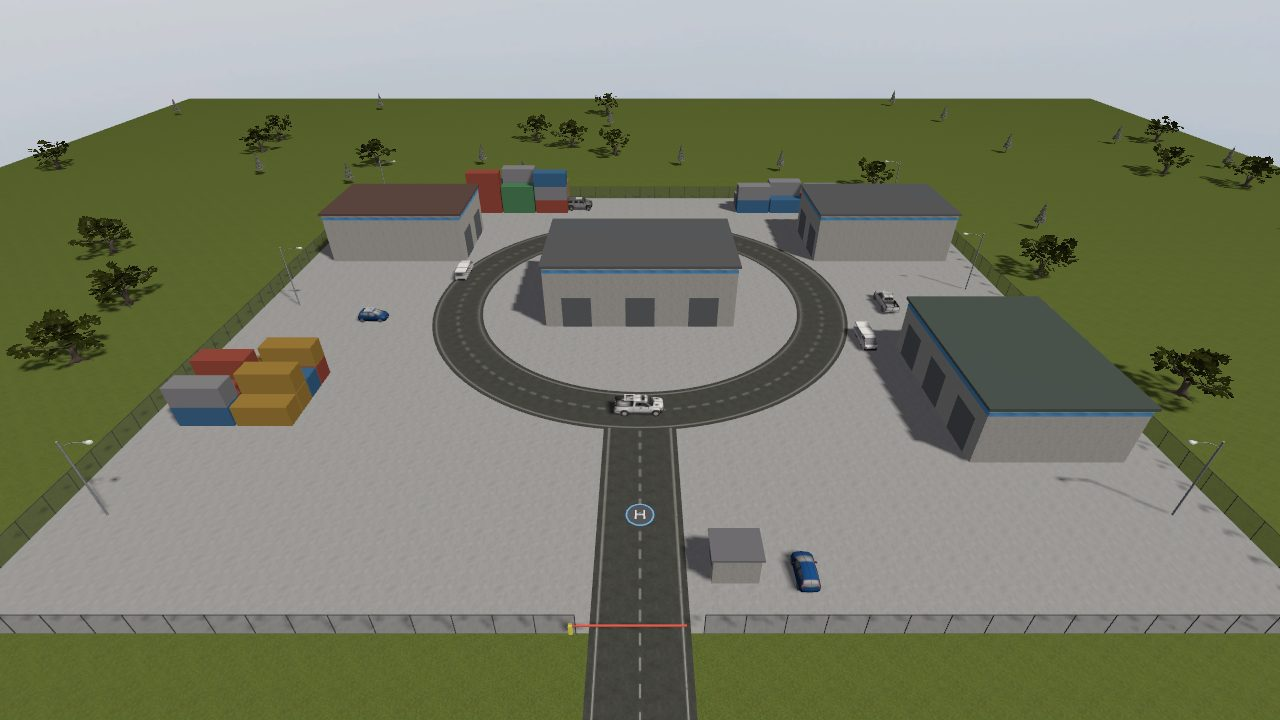
\includegraphics[width=\linewidth]{zona_bodegas}
  \end{columns}
\end{frame}

\begin{frame}[fragile]{Herramientas del paquete}
  \begin{lstlisting}[style=bash,caption={En src/x500\_retos/tools (las dos últimas con el venv del repo, trae OpenCV)}]
python3 tools/build_worlds.py                 # regenerar todos los mundos
/data/vespo_ws/venv/bin/python tools/make_aruco.py      # texturas ArUco
/data/vespo_ws/venv/bin/python tools/render_world.py plaza_show /tmp/fotos \
    "aerea:0,-36,20,0,0.5,1.5708:1.5"      # foto sin abrir Gazebo
  \end{lstlisting}
  \small \cmd{render\_world.py} agrega cámaras al mundo, corre Gazebo sin ventana con su propio
  \cmd{GZ\_PARTITION} (no choca con una simulación abierta) y guarda un PNG por cámara. Así se
  hicieron todas las capturas de esta presentación.
\end{frame}

% =============================================================================
\section{Nivel 1: moverse bien}
% =============================================================================

% ----------------------------------------------------------------------------- 1
\begin{frame}{Misión 1: la estrella del show}
  \begin{columns}[c]
    \column{0.5\textwidth}
    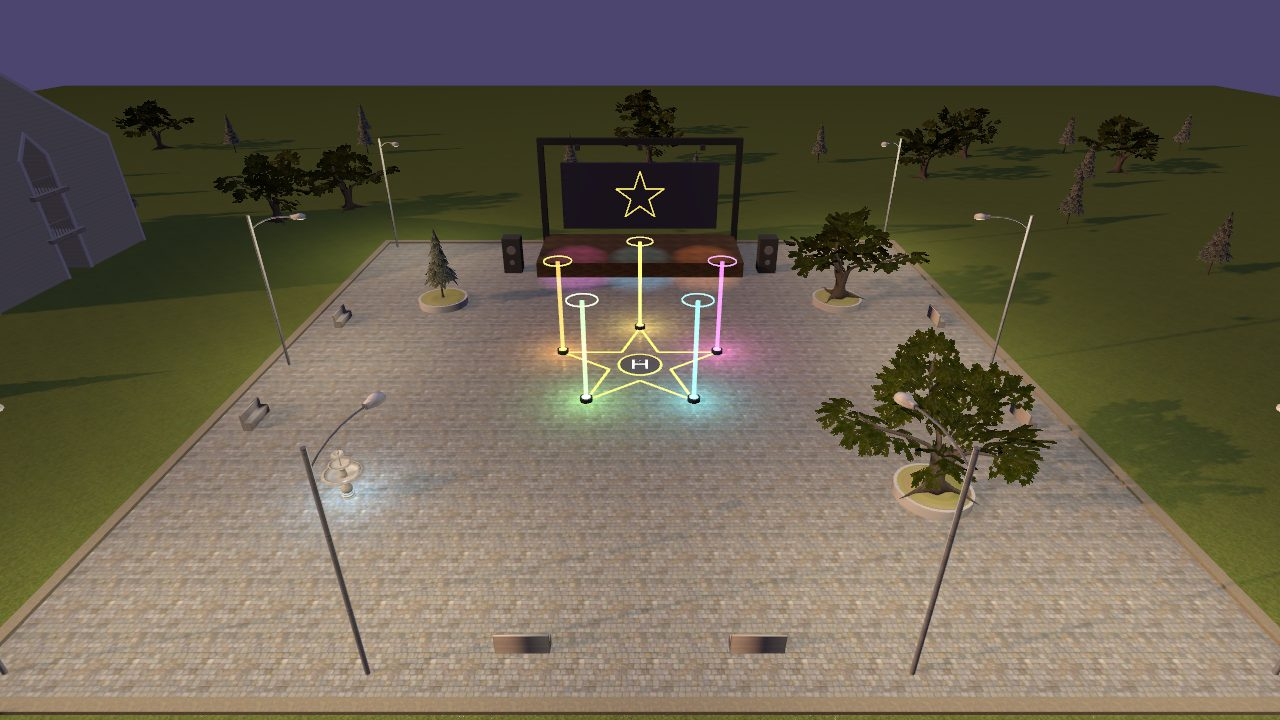
\includegraphics[width=\linewidth]{plaza_show}
    \column{0.47\textwidth}\small
    \textbf{Escenario}: una empresa de espectáculos quiere una estrella de 5 picos a 6 m de altura
    para el show de año nuevo.
    \begin{itemize}
      \item Mundo \cmd{plaza\_show}: la estrella dorada pintada en el piso.
      \item En cada pico, una baliza con un \textbf{aro a 6 m}: el dron tiene que pasar por adentro.
      \item \textbf{Viene de}: \cmd{square\_mission} (waypoints en offboard).
      \item \textbf{Lo nuevo}: los waypoints se \textbf{generan con una fórmula}.
    \end{itemize}
  \end{columns}
\end{frame}

\begin{frame}{La geometría de la estrella}
  \begin{columns}[c]
    \column{0.45\textwidth}\centering
    \begin{tikzpicture}[scale=0.42]
      \def\R{5} \def\r{1.91}
      \draw[gray!40] (0,0) circle (\R);
      \draw[gray!40,dashed] (0,0) circle (\r);
      \foreach \k in {0,...,4} {
        \pgfmathsetmacro{\a}{90-72*\k}
        \pgfmathsetmacro{\b}{90-72*\k-36}
        \coordinate (P\k) at (\a:\R);
        \coordinate (I\k) at (\b:\r);
      }
      \draw[naranja,thick] (P0)--(I0)--(P1)--(I1)--(P2)--(I2)--(P3)--(I3)--(P4)--(I4)--cycle;
      \foreach \k in {0,...,4} {\fill[azul] (P\k) circle (4pt); \fill[verde] (I\k) circle (3pt);}
      \node[above,font=\tiny] at (P0) {P0 (norte)};
      \node[right,font=\tiny] at (P1) {P1};
      \node[font=\tiny,right] at (I0) {I0};
      \draw[-{Stealth}] (0,0) -- (P0) node[midway,left,font=\tiny] {R};
      \fill (0,0) circle (2pt);
    \end{tikzpicture}
    \column{0.52\textwidth}\small
    \begin{itemize}
      \item \textbf{Picos} $P_k$: en el círculo de radio $R$, repartidos cada $360^\circ/N$, el primero
        al \textbf{norte}.
      \item \textbf{Interiores} $I_k$: en el círculo de radio $R\cdot$\cmd{inner\_ratio}, a medio
        camino (en ángulo) entre dos picos.
      \item Orden de vuelo: $P_0, I_0, P_1, I_1, \ldots$ y de vuelta a $P_0$.
      \item \cmd{inner\_ratio = 0.382}: estrella regular de 5.\\
        \cmd{inner\_ratio = 0}: polígono. Con \cmd{points:=4} debe salir \textbf{un cuadrado}.
    \end{itemize}
  \end{columns}
\end{frame}

\begin{frame}{Un punto en polares, en NED}
  \begin{columns}[c]
    \column{0.45\textwidth}\centering
    \begin{tikzpicture}[scale=1.1]
      \draw[-{Stealth},verde] (0,0) -- (0,2.2) node[above,font=\scriptsize] {N (x)};
      \draw[-{Stealth},rojo] (0,0) -- (2.2,0) node[right,font=\scriptsize] {E (y)};
      \draw[thick,azul] (0,0) -- (55:1.9);
      \fill[azul] (55:1.9) circle (2pt);
      \draw[-{Stealth}] (0,0.7) arc (90:55:0.7);
      \node[font=\scriptsize] at (0.45,0.95) {$a$};
      \node[font=\scriptsize,azul] at (1.6,1.75) {$(r\cos a,\ r\sin a)$};
    \end{tikzpicture}
    \column{0.52\textwidth}\small
    Con el ángulo $a$ medido \textbf{desde el norte, hacia el este}:
    \[ \text{norte} = r\cos a \qquad \text{este} = r\sin a \]
    \begin{ojo}
      \small Es al revés de la trigonometría de la escuela (desde el eje x, antihorario). Aquí
      $a = 0$ es el norte y $a = 90^\circ$ el este, porque así mide PX4 el yaw.
    \end{ojo}
  \end{columns}
\end{frame}

\begin{frame}[fragile]{Tu parte: \texttt{vertices()}}
  \begin{lstlisting}[style=cpp,caption={Lo que trae el reto (estrella\_show.cpp)}]
std::vector<Point> vertices() const {
  std::vector<Point> out;
  const float z = static_cast<float>(-altitude_);
  // TODO 1: los picos. Hay points_ picos repartidos en 360°, el primero al
  //   norte. ... Pista: el ángulo del pico k es 2*pi*k / points_ (en radianes).
  // TODO 2: los vértices interiores. Si inner_ratio_ > 0, después de cada
  //   pico va un vértice a radio radius_ * inner_ratio_, ...
  // Para agregar un punto:  out.push_back({norte, este, z});
  return out;
}
  \end{lstlisting}
  \small Si \cmd{vertices()} regresa la lista vacía, el nodo despega, avisa y aterriza.
\end{frame}

\begin{frame}{Cómo vuela y cómo se califica}
  \begin{columns}[c]
    \column{0.5\textwidth}
    \begin{tikzpicture}[node distance=0.35cm,st/.style={draw=azul,fill=azulclaro,rounded corners,font=\tiny,minimum width=1.4cm}]
      \node[st] (a) {WARMUP}; \node[st,below=of a] (b) {TAKEOFF};
      \node[st,below=of b,fill=yellow!20] (c) {STAR};
      \node[st,below=of c] (d) {CENTER}; \node[st,below=of d] (e) {LANDING};
      \draw[-{Stealth}] (a)--(b); \draw[-{Stealth}] (b)--node[right,font=\tiny]{al centro, a 6 m}(c);
      \draw[-{Stealth}] (c)--node[right,font=\tiny]{último vértice}(d); \draw[-{Stealth}] (d)--(e);
      \draw[-{Stealth}] (c.west) to[bend left=60] node[left,font=\tiny,align=right]{a \textless0.5 m:\\0.5 s quieto,\\siguiente} (c.west|-c.north);
    \end{tikzpicture}
    \column{0.47\textwidth}
    \begin{terminal}{al aterrizar}
Qué tan cerca pasó de cada vértice:\\
\ \ 1: 0.15 m OK\\
\ \ 2: 0.11 m OK\\
\ \ ...\\
\ 11: 0.05 m OK\\
Misión cumplida
    \end{terminal}
    \small\textbf{Éxito}: pasa a menos de \cmd{tolerance} (0.5 m) de cada vértice, regresa al centro y aterriza.
  \end{columns}
\end{frame}

\begin{frame}{Errores típicos en la misión 1}
  \begin{itemize}\small
    \item \textbf{Radianes vs grados}: \cmd{std::cos} recibe radianes. $2\pi k/N$, no $360k/N$.
    \item \textbf{División entera}: \cmd{2 * M\_PI * k / points\_} está bien; \cmd{k / points\_ * 2 * M\_PI} da 0
      (\cmd{k} y \cmd{points\_} son enteros).
    \item \textbf{double a float}: \cmd{Point} es \cmd{std::array<float,3>}; usen \cmd{static\_cast<float>()}.
    \item \textbf{Cerrar la figura}: el último punto debe ser otra vez el pico 0.
    \item \textbf{z positiva}: si el dron se va al suelo, les faltó el signo menos.
  \end{itemize}
  \begin{idea}
    \small Prueben \cmd{points:=6}, \cmd{points:=4 inner\_ratio:=0.0} (cuadrado) y \cmd{radius:=3.0}:
    un buen generador funciona para cualquier N.
  \end{idea}
\end{frame}

% ----------------------------------------------------------------------------- 2
\begin{frame}{Misión 2: inspección de un pilar}
  \begin{columns}[c]
    \column{0.5\textwidth}
    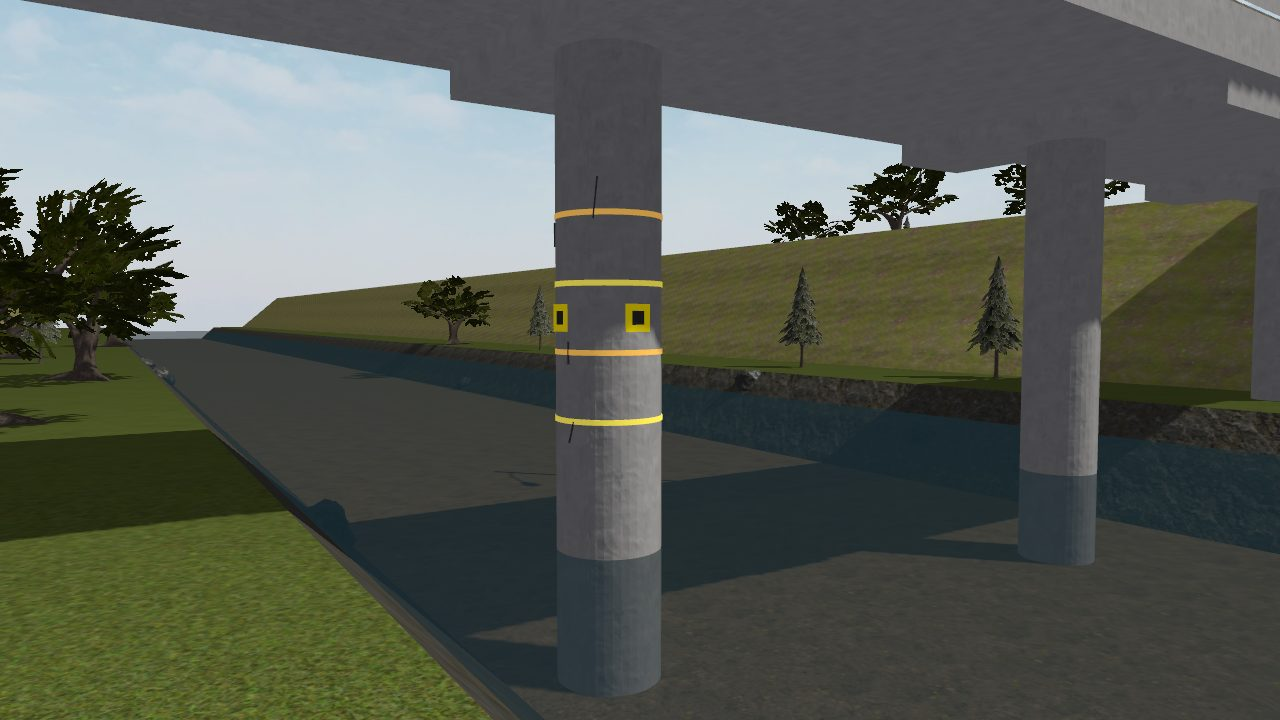
\includegraphics[width=\linewidth]{puente_rio_pilar}
    \column{0.47\textwidth}\small
    \textbf{Escenario}: una constructora necesita fotos de un pilar de puente desde todos los
    ángulos y alturas.
    \begin{itemize}
      \item Subir en \textbf{hélice} alrededor del pilar: 3 vueltas de 1 m a 4 m.
      \item La nariz (la cámara) \textbf{siempre apuntando al pilar}.
      \item \textbf{Viene de}: \cmd{orbit\_mission} + \cmd{figure\_eight}.
      \item Las bandas de colores del pilar están justo a 1, 2, 3 y 4 m.
    \end{itemize}
  \end{columns}
\end{frame}

\begin{frame}{La hélice: un círculo que sube}
  \begin{columns}[c]
    \column{0.45\textwidth}\centering
    \begin{tikzpicture}[scale=0.85]
      \draw[thick,fill=gray!30] (-0.25,0) rectangle (0.25,3.2);
      \draw[azul,thick,domain=0:1080,samples=200,smooth,variable=\t]
        plot ({1.3*cos(\t)}, {0.3+0.0024*\t + 0.25*sin(\t)});
      \node[font=\tiny,right] at (1.4,0.3) {1 m: entra};
      \node[font=\tiny,right] at (1.4,2.9) {4 m: sale};
      \draw[-{Stealth},dashed] (0,-0.3) -- (1.3,-0.3) node[midway,below,font=\tiny] {radio 3 m};
    \end{tikzpicture}
    \column{0.52\textwidth}\small
    Con velocidad angular $\omega = v/R$ y empezando en el ángulo $\theta_0$:
    \[ \theta(t) = \theta_0 + \omega t \]
    \[ N(t) = N_c + R\cos\theta(t) \qquad E(t) = E_c + R\sin\theta(t) \]
    y la altura \textbf{sube lineal} de \cmd{z\_start} a \cmd{z\_end} en la duración total
    $T = \text{vueltas}\cdot 2\pi R / v$.
    \vspace{0.3em}

    \footnotesize $\theta_0$ es el punto del círculo más cercano al despegue: así llega sin rodear el pilar.
  \end{columns}
\end{frame}

\begin{frame}{Derivar para el feedforward}
  \small \cmd{figure\_eight} ya lo hace con su curva: la velocidad es la derivada de la posición.
  Para un círculo:
  \[
    \frac{d}{dt}\bigl(R\cos\theta(t)\bigr) = -R\,\omega\sin\theta(t)
    \qquad
    \frac{d}{dt}\bigl(R\sin\theta(t)\bigr) = R\,\omega\cos\theta(t)
  \]
  \begin{columns}[c]
    \column{0.55\textwidth}
    \begin{itemize}
      \item La velocidad es \textbf{tangente} al círculo, de magnitud $R\omega = v$.
      \item La aceleración (segunda derivada) apunta \textbf{al centro}, de magnitud $R\omega^2$.
      \item Y en $z$: si sube lineal, ¿cuánto vale $dz/dt$? (cuidado: NED, arriba es $-z$).
    \end{itemize}
    \column{0.42\textwidth}
    \begin{tikzpicture}[scale=0.8]
      \draw[gray] (0,0) circle (1.4);
      \fill (40:1.4) circle (2pt);
      \draw[-{Stealth},azul,thick] (40:1.4) -- ++(130:0.9) node[above,font=\tiny] {$v$};
      \draw[-{Stealth},rojo,thick] (40:1.4) -- (40:0.6) node[below,font=\tiny] {$a$};
      \fill (0,0) circle (1.5pt);
    \end{tikzpicture}
  \end{columns}
\end{frame}

\begin{frame}{Apuntar al pilar}
  \begin{columns}[c]
    \column{0.45\textwidth}\centering
    \begin{tikzpicture}[scale=0.9]
      \draw[gray] (0,0) circle (1.5);
      \fill[gray!60] (0,0) circle (0.3);
      \fill[azul] (130:1.5) circle (3pt);
      \draw[-{Stealth},thick,naranja] (130:1.5) -- (130:0.4) node[midway,above,font=\tiny,sloped] {nariz};
      \draw[-{Stealth},verde] (0,0) -- (0,2) node[above,font=\tiny] {N};
      \draw[-{Stealth},rojo] (0,0) -- (2,0) node[right,font=\tiny] {E};
    \end{tikzpicture}
    \column{0.52\textwidth}\small
    El yaw que apunta del dron al centro es el ángulo del vector \emph{dron $\rightarrow$ centro}:
    \[ \psi = \operatorname{atan2}(E_c - E,\ N_c - N) \]
    (\cmd{atan2(este, norte)}: el orden importa).
    \vspace{0.3em}

    Y \cmd{yawspeed} = qué tan rápido gira esa dirección: en un círculo, lo mismo que $\omega$.
  \end{columns}
\end{frame}

\begin{frame}{Cómo se califica la hélice}
  \small Mientras vuela, el nodo mide contra la \textbf{posición real} (no contra el setpoint):
  \begin{columns}[c]
    \column{0.55\textwidth}
    \begin{itemize}
      \item \textbf{Radio}: distancia real al eje del pilar, dentro de $3 \pm 0.3$ m.
      \item \textbf{Yaw}: la nariz contra la dirección real al pilar, error $< 10^\circ$.
      \item \textbf{Vueltas}: suma del ángulo recorrido alrededor del pilar $\geq$ 90\% de 3.
      \item \textbf{Altura}: llegó a \cmd{z\_end} (4 m) $- 0.3$.
    \end{itemize}
    \column{0.42\textwidth}
    \begin{terminal}{al aterrizar}
vueltas: 2.99 de 3.00 OK\\
altura máxima: 3.99 m OK\\
error de radio: 0.11 m OK\\
error de yaw: 6.1° OK\\
Misión cumplida
    \end{terminal}
  \end{columns}
\end{frame}

\begin{frame}{El extra: arrancar suave}
  \begin{columns}[c]
    \column{0.55\textwidth}\small
    Si todo pasa menos el yaw, que se pasa de 10° \textbf{justo al empezar}:
    \begin{itemize}
      \item En $t = 0$ la velocidad del setpoint salta de 0 a $v$ en un instante.
      \item El dron no puede acelerar infinito: se queda atrás un momento.
      \item El setpoint ya va adelante y la nariz apunta a donde \emph{debería} estar, no a donde está.
    \end{itemize}
    Pista: que la velocidad suba de 0 a $v$ en 1--2 s (y no olviden sumar ese tiempo a la duración).
    \column{0.42\textwidth}
    \begin{tikzpicture}[x=0.6cm,y=0.9cm]
      \draw[-{Stealth}] (0,0) -- (5.5,0) node[right,font=\tiny] {t};
      \draw[-{Stealth}] (0,0) -- (0,1.6) node[above,font=\tiny] {v};
      \draw[rojo,thick] (0,0) -- (0,1.2) -- (5,1.2);
      \draw[verde,thick,domain=0:5,samples=40] plot (\x,{1.2*(1-exp(-\x/0.8))});
      \node[font=\tiny,rojo] at (3.3,1.4) {escalón};
      \node[font=\tiny,verde] at (3.3,0.8) {rampa};
    \end{tikzpicture}
  \end{columns}
\end{frame}

% ----------------------------------------------------------------------------- 3
\begin{frame}{Misión 3: entrega a domicilio}
  \begin{columns}[c]
    \column{0.5\textwidth}
    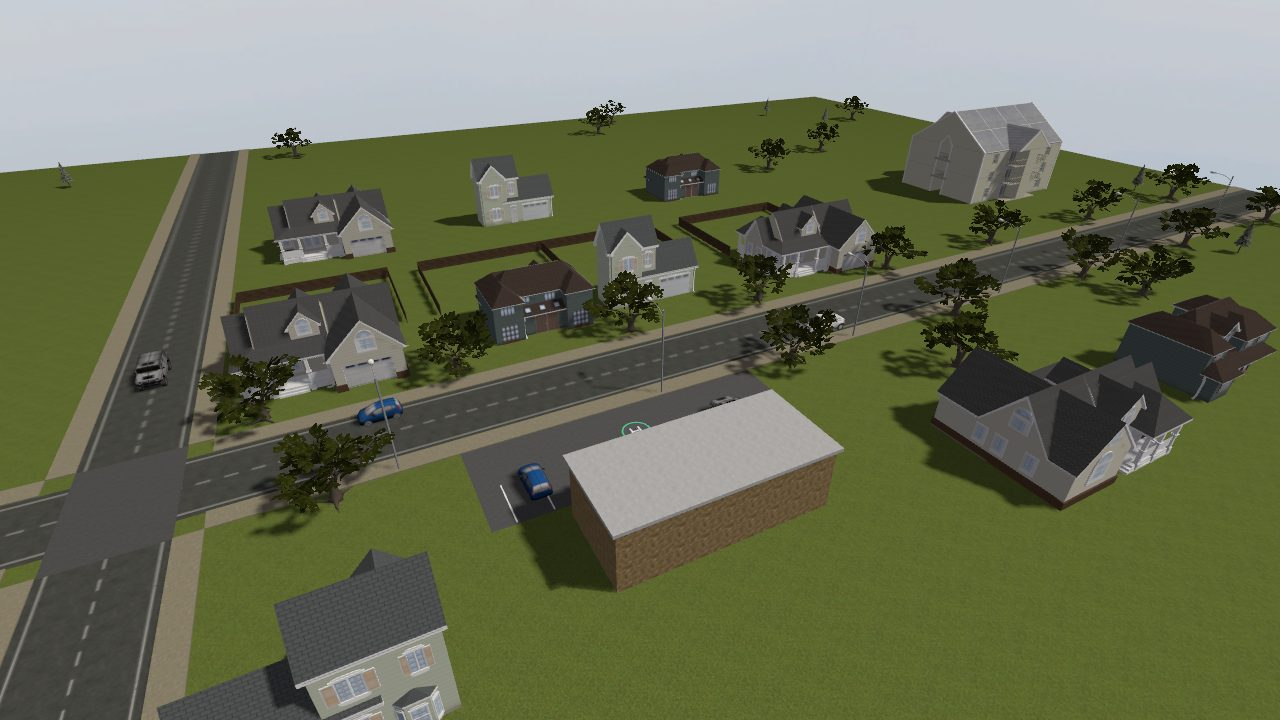
\includegraphics[width=\linewidth]{barrio_entrega}
    \column{0.47\textwidth}\small
    \textbf{Escenario}: llevar un medicamento de la farmacia a una casa a \textasciitilde40 m,
    dejarlo y volver solo.
    \begin{itemize}
      \item \textbf{Sin offboard}: PX4 vuela cada tramo con sus modos; el nodo solo decide qué sigue.
      \item Si el nodo se muere, el dron se queda en Hold (no hay failsafe de offboard).
      \item \textbf{Viene de}: \cmd{goto\_mission} + \cmd{return\_home} + \cmd{set\_home}.
    \end{itemize}
  \end{columns}
\end{frame}

\begin{frame}{Las fases (el log las numera [1/9] \ldots{} [9/9])}
  \centering
  \begin{tikzpicture}[node distance=0.25cm,st/.style={draw=azul,fill=azulclaro,rounded corners,font=\tiny,minimum width=1.8cm,minimum height=0.45cm,align=center}]
    \node[st] (1) {WAIT\_GPS};
    \node[st,right=of 1] (2) {ARMING};
    \node[st,right=of 2] (3) {TAKEOFF};
    \node[st,right=of 3] (4) {FLY};
    \node[st,right=of 4] (5) {LAND\_DEST};
    \node[st,below=0.9cm of 5,fill=yellow!20] (6) {DELIVER};
    \node[st,left=of 6,fill=yellow!20] (7) {REARM};
    \node[st,left=of 7,fill=yellow!20] (8) {TAKEOFF\_BACK};
    \node[st,left=of 8,fill=yellow!20] (9) {SET\_HOME};
    \node[st,left=of 9,fill=yellow!20] (10) {RETURN};
    \foreach \a/\b in {1/2,2/3,3/4,4/5,5/6,6/7,7/8,8/9,9/10} \draw[-{Stealth}] (\a) -- (\b);
  \end{tikzpicture}
  \vspace{0.5em}
  \begin{columns}[t]
    \column{0.5\textwidth}\small
    \textbf{Ya funciona}: de la farmacia hasta aterrizar en el patio (azul).
    \column{0.47\textwidth}\small
    \textbf{Tu parte} (amarillo): esperar desarmado, volver a armar y despegar, \textbf{arreglar casa}
    y regresar con Return.
  \end{columns}
\end{frame}

\begin{frame}[fragile]{Las ayudas que ya están hechas}
  \begin{lstlisting}[style=cpp,caption={entrega\_domicilio: tu trabajo es decidir CUÁNDO llamar cada una}]
bool arm_when_ready();        // Hold y armar, reintentando cada 1 s; true si ya armó
void take_off();              // NAV_TAKEOFF sobre donde está, a cruise_alt
void go_to_target();          // DO_REPOSITION al patio: vuela y queda en Hold
void set_home_to_pharmacy();  // DO_SET_HOME con las coordenadas de la farmacia
bool at_cruise_alt() const;   // en Hold y a la altura de crucero
double home_offset() const;   // qué tan lejos de la farmacia está "casa"
  \end{lstlisting}
  \small Y \cmd{px4\_.home().update\_count}: sube cada vez que PX4 mueve ``casa''
  (así sabes que aceptó el \cmd{DO\_SET\_HOME}, como en \cmd{set\_home.cpp}).
\end{frame}

\begin{frame}{La trampa: ¿dónde quedó casa?}
  \begin{columns}[c]
    \column{0.5\textwidth}\small
    PX4 fija ``casa'' \textbf{donde arma}.
    \begin{enumerate}
      \item Arma en la farmacia $\Rightarrow$ casa = farmacia.
      \item Aterriza en el patio y desarma.
      \item \textbf{Vuelve a armar en el patio} $\Rightarrow$ casa = \ldots
    \end{enumerate}
    Si mandan Return así, ¿a dónde regresa?
    \vspace{0.3em}
    \begin{idea}
      \small El nodo guarda las coordenadas de la farmacia al principio
      (\cmd{pharmacy\_lat\_}, \cmd{pharmacy\_lon\_}). \cmd{px4\_.home()} les dice dónde cree PX4
      que está casa.
    \end{idea}
    \column{0.47\textwidth}
    \begin{tikzpicture}[scale=0.8]
      \node[draw,fill=green!20,font=\tiny] (f) at (0,0) {farmacia (H)};
      \node[draw,fill=orange!30,font=\tiny] (p) at (3,3) {patio};
      \draw[-{Stealth},thick,azul] (f) to[bend left] node[above left,font=\tiny] {ida} (p);
      \draw[-{Stealth},thick,verde,dashed] (p) to[bend left] node[below right,font=\tiny] {Return correcto} (f);
      \draw[-{Stealth},thick,rojo] (p.east) .. controls (4.6,3.6) and (4.2,2.2) .. node[right,font=\tiny] {Return con casa en el patio} (p.south east);
    \end{tikzpicture}
  \end{columns}
\end{frame}

\begin{frame}{Alturas y GPS en la entrega}
  \small
  \begin{itemize}
    \item La plataforma está en \textbf{lat 47.3982949, lon 8.5463757} (36 m N, 16 m E de la farmacia).
    \item La ruta directa pasa \textbf{sobre la casa destino}, de \textasciitilde9 m: \cmd{cruise\_alt}
      tiene que librarla (15 m por defecto).
    \item Los comandos piden altura \textbf{AMSL} (sobre el nivel del mar): el nodo guarda la altura del
      suelo al principio y le suma \cmd{cruise\_alt}.
    \item \cmd{Return} sube primero a \cmd{RTL\_RETURN\_ALT} (30 m en el x500 de SITL), vuela a casa y baja.
  \end{itemize}
  \begin{terminal}{al aterrizar en la farmacia}
De vuelta en la farmacia y desarmado. Misión de 119 s\\
\ \ a 0.01 m de la H OK\\
Misión cumplida
  \end{terminal}
\end{frame}

% =============================================================================
\section{Nivel 2: decidir solo}
% =============================================================================

% ----------------------------------------------------------------------------- 4
\begin{frame}{Misión 4: la geocerca del concierto}
  \begin{columns}[c]
    \column{0.5\textwidth}
    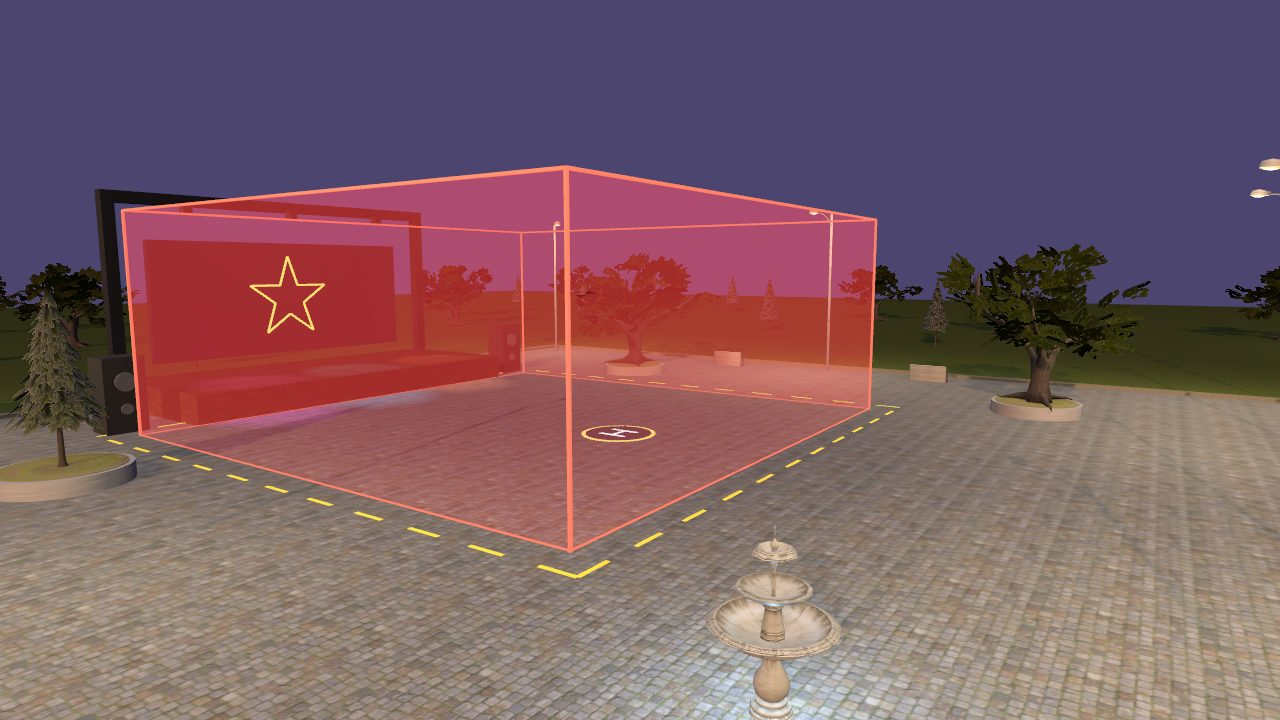
\includegraphics[width=\linewidth]{plaza_concierto}
    \column{0.47\textwidth}\small
    \textbf{Escenario}: en un concierto el dron no puede salirse de una caja de
    20\,$\times$\,20\,$\times$\,8 m.
    \begin{itemize}
      \item Un nodo \textbf{guardián} que \textbf{no vuela}: solo vigila.
      \item Si el dron va a salirse: \textbf{Hold}, y ya quieto, \textbf{Return}.
      \item Funciona \textbf{sin importar quién vuela}: un nodo, QGC o un piloto.
      \item \textbf{Viene de}: \cmd{flight\_mode\_monitor} + \cmd{return\_home}.
    \end{itemize}
  \end{columns}
\end{frame}

\begin{frame}{La caja}
  \begin{columns}[c]
    \column{0.47\textwidth}\centering
    \begin{tikzpicture}[scale=0.17]
      \draw[orange,dashed,thick] (-11,-7) rectangle (11,15);
      \draw[rojo,thick,fill=red!8] (-10,-6) rectangle (10,14);
      \fill[gray!40] (-8,14) rectangle (8,21);
      \node[font=\tiny] at (0,17.5) {escenario};
      \node[draw,circle,fill=azulclaro,inner sep=0.5pt,font=\tiny] at (0,0) {H};
      \draw[-{Stealth}] (0,0) -- (0,4) node[above,font=\tiny] {N};
      \node[font=\tiny,rojo] at (6,-4.5) {zona permitida};
      \node[font=\tiny,orange] at (6,-8.7) {límite +1 m};
    \end{tikzpicture}
    \column{0.5\textwidth}\small
    En NED desde el despegue (parámetros del nodo):
    \begin{center}
      \begin{tabular}{ll}
        \toprule
        norte & $-6 \ldots 14$ m \\
        este  & $-10 \ldots 10$ m \\
        altura & hasta 8 m \\
        \bottomrule
      \end{tabular}
    \end{center}
    Las paredes rojas son solo visuales: el dron las atraviesa. La \textbf{línea naranja punteada}
    del piso está 1 m afuera: es el criterio de éxito.
  \end{columns}
\end{frame}

\begin{frame}{¿Por qué no basta con revisar si ya se salió?}
  \begin{columns}[c]
    \column{0.52\textwidth}\small
    El dron \textbf{no frena en seco}. Desde que el guardián detecta hasta que el dron se detiene:
    \[ d = \underbrace{v\,t_r}_{\text{reacción}} + \underbrace{\frac{v^2}{2a}}_{\text{frenado}} \]
    Medido en SITL: a 4 m/s el x500 en Hold recorre todavía \textasciitilde4.5 m
    (frena a \textasciitilde2.4 m/s$^2$).
    \vspace{0.3em}
    \begin{idea}
      \small Hay que \textbf{predecir} dónde se va a detener y actuar si \emph{ese} punto queda fuera.
    \end{idea}
    \column{0.45\textwidth}
    \begin{tikzpicture}[x=0.5cm,y=0.5cm]
      \draw[rojo,thick] (8,-1) -- (8,3) node[above,font=\tiny] {cerca};
      \draw[orange,dashed] (9,-1) -- (9,3) node[above,font=\tiny] {+1 m};
      \fill[azul] (2,1) circle (4pt) node[below,font=\tiny] {ahora};
      \draw[-{Stealth},azul] (2,1) -- (3.6,1);
      \fill[gray] (5,1) circle (3pt) node[below,font=\tiny,align=center] {detenido\\(predicción)};
      \draw[decorate,decoration={brace,amplitude=4pt}] (2,1.6) -- (5,1.6) node[midway,above=3pt,font=\tiny] {$v t_r + v^2/2a$};
    \end{tikzpicture}
  \end{columns}
\end{frame}

\begin{frame}{Prueba de la fórmula}
  \small Frenando con aceleración constante $a$ desde $v$:
  \[ v(t) = v - a t \;\Rightarrow\; t_{\text{alto}} = \frac{v}{a}
     \qquad
     d = v\,t_{\text{alto}} - \tfrac12 a\,t_{\text{alto}}^2 = \frac{v^2}{a} - \frac{v^2}{2a} = \frac{v^2}{2a} \]
  \centering
  \begin{tabular}{rrr}
    \toprule
    $v$ (m/s) & $d$ con $a = 2$ m/s$^2$, $t_r = 0.5$ s & lo que hay que anticipar \\
    \midrule
    2 & $1.0 + 1.0 = 2.0$ m & poco \\
    4 & $2.0 + 4.0 = 6.0$ m & más que la tolerancia \\
    6 & $3.0 + 9.0 = 12.0$ m & más de la mitad de la caja \\
    \bottomrule
  \end{tabular}
  \vspace{0.4em}

  \raggedright\footnotesize Por eso \cmd{brake\_accel} = 2.0 y \cmd{reaction} = 0.5 por defecto: un poco más conservador que lo medido.
\end{frame}

\begin{frame}[fragile]{Tu parte en el guardián}
  \begin{lstlisting}[style=cpp,caption={guardian\_geocerca: los tres TODO}]
Vec3 stop_point() const {          // TODO 1: dónde se detendría
  // cada eje avanza  v * reaction_  +  v * |v| / (2 a)   (v*|v| conserva el signo)
}
case State::WATCH:                 // TODO 2: si stop_point() queda afuera
  // (outside_by(...) > 0): px4_.request_hold(), avisar y pasar a BRAKING
case State::BRAKING:               // TODO 3: casi quieto (speed() < 0.3) y en Hold:
  // px4_.return_home() y RETURNING. Si en 1 s no entró a Hold, pedirlo otra vez.
  \end{lstlisting}
  \small Ya hechos: \cmd{outside\_by(p)} (cuánto está afuera un punto), \cmd{speed()},
  \cmd{distance\_to\_edge()} y la medición de cuánto se salió.
\end{frame}

\begin{frame}[fragile]{Probarlo: el piloto travieso}
  \begin{lstlisting}[style=bash,caption={Tres terminales}]
vespo up --sim --world plaza_concierto
ros2 run x500_retos guardian_geocerca
ros2 run x500_retos vuelo_prueba --ros-args -p direction_deg:=0.0 -p speed:=6.0
  \end{lstlisting}
  \begin{columns}[c]
    \column{0.5\textwidth}\small
    \cmd{vuelo\_prueba} (ya completo) despega y se lanza en línea recta sin frenar, hasta que
    alguien le quite el control o llegue a \cmd{max\_distance} (30 m, red de seguridad).
    \vspace{0.3em}

    \cmd{direction\_deg}: 0 = norte (hay 14 m para acelerar), 90 = este, 180 = sur.
    \column{0.47\textwidth}
    \begin{terminal}{guardian\_geocerca}
¡Se va a salir! (a 5.1 m de la\\
\ orilla, va a 5.5 m/s): Hold\\
Detenido a 0.00 m fuera. Return\\
Lo más que se salió: 0.00 m OK
    \end{terminal}
  \end{columns}
\end{frame}

\begin{frame}{Un detalle de la vida real: Return se sale por arriba}
  \begin{columns}[c]
    \column{0.55\textwidth}\small
    Return sube primero a \cmd{RTL\_RETURN\_ALT} (30 m en el x500 de SITL, recortado por un cono
    cerca de casa). En la prueba subió a 9 m: \textbf{arriba de la caja}.
    \vspace{0.3em}

    El guardián no lo cuenta como falla suya (es configuración de PX4), pero avisa:
    \begin{terminal}{guardian\_geocerca}
Return subió a 9 m, arriba de la cerca:\\
\ baja RTL\_RETURN\_ALT en QGC
    \end{terminal}
    \column{0.42\textwidth}
    \begin{idea}
      \small En un concierto real eso se configura antes de volar: QGC $\rightarrow$ Parámetros
      $\rightarrow$ Return Mode, por debajo del techo de la geocerca.
    \end{idea}
  \end{columns}
\end{frame}

% ----------------------------------------------------------------------------- 5
\begin{frame}{Misión 5: cruzar una cueva}
  \begin{columns}[c]
    \column{0.5\textwidth}
    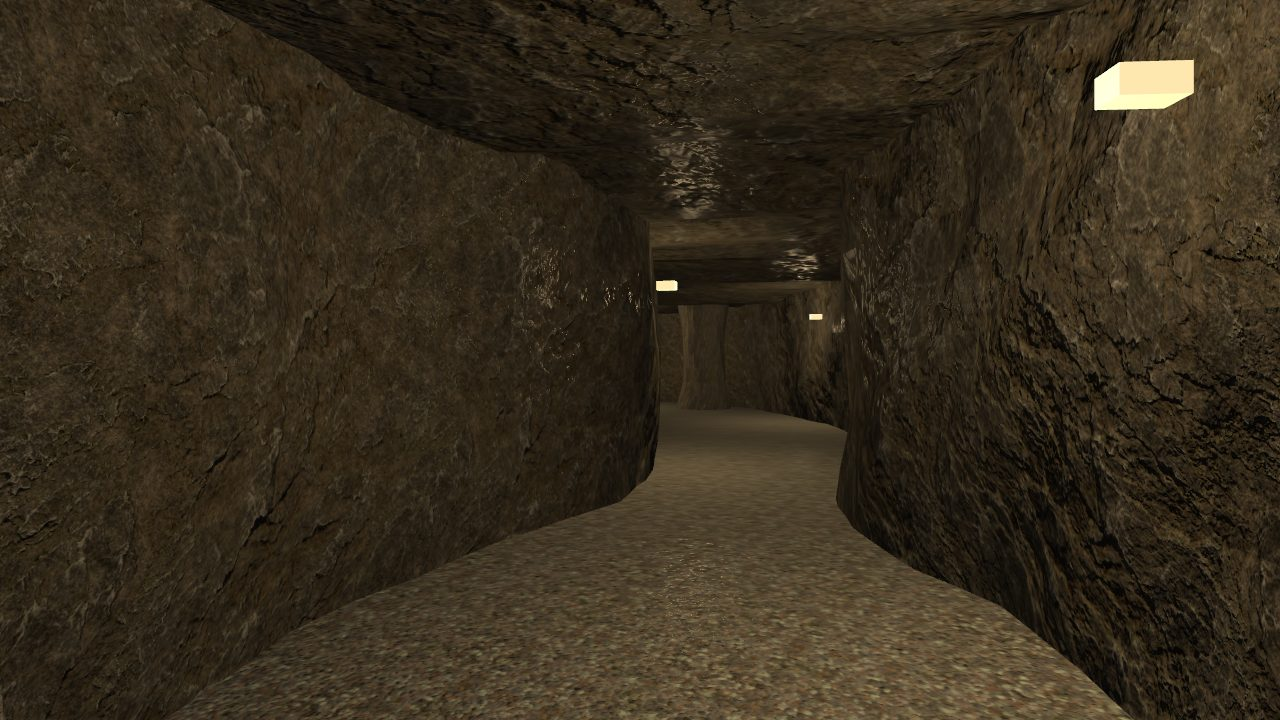
\includegraphics[width=\linewidth]{cueva_angostura}
    \column{0.47\textwidth}\small
    \textbf{Escenario}: atravesar un túnel curvo y oscuro usando \textbf{solo el lidar} para no chocar.
    \begin{itemize}
      \item Túnel de \textasciitilde66 m, 5 m de ancho, 4 m de alto.
      \item Dos angosturas de 3 m.
      \item Una columna de roca a medio camino: \textbf{solo se pasa por la izquierda}.
      \item \textbf{Viene de}: \cmd{velocity\_control}.
    \end{itemize}
  \end{columns}
\end{frame}

\begin{frame}{El mapa de la cueva}
  \centering
  \begin{tikzpicture}[x=0.12cm,y=0.09cm]
    \draw[gray!50,fill=gray!15] (-40,10) rectangle (40,76);
    \node[font=\tiny,gray] at (-28,70) {loma};
    \draw[azul,line width=3.5pt,opacity=0.5,smooth] plot coordinates {(0,10) (0,16) (2,23) (6,30) (8,37) (7,44) (3,50) (-1,56) (-3,63) (-2,70) (-1,76)};
    \draw[azul,thick,smooth] plot coordinates {(0,0) (0,10) (0,16) (2,23) (6,30) (8,37) (7,44) (3,50) (-1,56) (-3,63) (-2,70) (-1,76) (-1,84)};
    \node[draw,circle,fill=azulclaro,inner sep=0.5pt,font=\tiny] at (0,0) {H};
    \fill[orange] (-2.5,81.5) rectangle (0.5,86.5); \node[font=\tiny,right] at (1,84) {plataforma (N 84, E $-$1)};
    \fill[gray!70] (5.5,34) circle (1.5); \node[font=\tiny,right] at (9,34) {columna};
    \node[font=\tiny,right] at (4,23) {angostura};
    \node[font=\tiny,right] at (3,55) {angostura};
    \node[font=\tiny,right] at (1,11.5) {boca sur (N 10)};
    \node[font=\tiny,right] at (1,74.5) {boca norte (N 76)};
  \end{tikzpicture}
\end{frame}

\begin{frame}{El lidar 2D: \texttt{sensor\_msgs/LaserScan}}
  \begin{columns}[c]
    \column{0.45\textwidth}\centering
    \begin{tikzpicture}[scale=1]
      \fill[azul!10] (0,0) -- (-135+90:2) arc (-45:225:2) -- cycle;
      \foreach \a in {-120,-90,...,120} \draw[azul!40] (0,0) -- (\a+90:2);
      \draw[thick,fill=gray!30] (-0.25,-0.25) rectangle (0.25,0.25);
      \draw[-{Stealth},thick] (0,0.25) -- (0,0.9);
      \node[font=\tiny] at (0,2.25) {0° (frente)};
      \node[font=\tiny] at (-2.35,0) {+90° (izq)};
      \node[font=\tiny] at (2.35,0) {$-$90° (der)};
      \node[font=\tiny] at (0,-0.6) {$\pm$135° (atrás: ciego)};
    \end{tikzpicture}
    \column{0.52\textwidth}\small
    \begin{itemize}
      \item 1080 rayos de \cmd{angle\_min} $= -135^\circ$ a $+135^\circ$, cada \cmd{angle\_increment}.
      \item \cmd{ranges[i]}: distancia del rayo $i$ (m). \textbf{inf} si no pega en nada (hasta 30 m).
      \item Ángulo del rayo: \cmd{angle\_min + i * angle\_increment}.
      \item Ángulos \textbf{positivos a la izquierda} (FLU, convención de ROS).
      \item Va arriba del dron: el plano de escaneo está \textasciitilde0.3 m sobre el cuerpo.
    \end{itemize}
  \end{columns}
\end{frame}

\begin{frame}[fragile]{De Gazebo a ROS: el puente}
  \begin{lstlisting}[style=bash,caption={Lo que hace cueva.launch.py}]
ros2 run ros_gz_bridge parameter_bridge \
  /world/cueva/model/x500_lidar_2d_0/link/link/sensor/lidar_2d_v2/scan@sensor_msgs/msg/LaserScan[gz.msgs.LaserScan
#  ...y lo renombra a /x500/scan
  \end{lstlisting}
  \small
  \begin{itemize}
    \item \cmd{[} = solo de Gazebo hacia ROS. (\cmd{]} sería de ROS a Gazebo, \cmd{@} en ambos sentidos.)
    \item El nombre del topic de Gazebo incluye el mundo y el modelo (\cmd{x500\_lidar\_2d\_0}).
    \item \cmd{ros2 launch x500\_retos cueva.launch.py} levanta el puente y tu nodo juntos.
  \end{itemize}
\end{frame}

\begin{frame}{La herramienta: el mínimo de un sector}
  \begin{columns}[c]
    \column{0.45\textwidth}\centering
    \begin{tikzpicture}[scale=0.9]
      \fill[verde!25] (0,0) -- (75:2.2) arc (75:105:2.2) -- cycle;
      \fill[naranja!30] (0,0) -- (150:2.2) arc (150:210:2.2) -- cycle;
      \fill[naranja!30] (0,0) -- (-30:2.2) arc (-30:30:2.2) -- cycle;
      \draw[thick,fill=gray!30] (-0.2,-0.2) rectangle (0.2,0.2);
      \node[font=\tiny] at (90:2.5) {frente: $-15..15$};
      \node[font=\tiny] at (180:2.7) {izq: $60..120$};
      \node[font=\tiny] at (0:2.7) {der: $-120..-60$};
    \end{tikzpicture}
    \column{0.52\textwidth}\small
    Ya hecha en el nodo:
    \begin{center}\cmd{sector\_min(from\_deg, to\_deg)}\end{center}
    La distancia \textbf{más corta} que ve el lidar entre dos ángulos (positivo = izquierda). Lo que no
    pega en nada cuenta como \cmd{range\_max}.
    \vspace{0.3em}

    \footnotesize En el dibujo los sectores están girados: el frente va hacia arriba.
  \end{columns}
\end{frame}

\begin{frame}{Tu parte: \texttt{steer()}, del scan a una velocidad}
  \small Se llama 20 veces por segundo. Regresa \cmd{forward}, \cmd{left} (m/s) y \cmd{yawrate} (rad/s):
  \begin{enumerate}
    \item \textbf{Centrarse}: compara izquierda contra derecha y muévete hacia el lado con más espacio,
      proporcional a la diferencia y con tope. Afuera de la cueva un lado da 30 m: usa
      \cmd{std::min(d, 3.0)} para que solo cuenten las paredes cercanas.
    \item \textbf{Girar con la cueva}: busca el ángulo entre $-75^\circ$ y $75^\circ$ con más espacio libre y gira
      hacia él. Mejor: el espacio de cada ángulo como el \textbf{mínimo de una ventana} de $\pm10^\circ$,
      para no meterte por una rendija donde no cabes.
    \item \textbf{Avanzar}: más rápido si el frente está libre, más lento si hay que girar mucho.
  \end{enumerate}
  \begin{idea}
    \small Ya hecho: si hay algo a menos de \cmd{stop\_distance} al frente, no avanza; si pasa
    \cmd{stuck\_time} sin moverse, aterriza ``atorado''.
  \end{idea}
\end{frame}

\begin{frame}{Buscar el hueco: ventanas, no rayos}
  \begin{columns}[c]
    \column{0.5\textwidth}\centering
    \begin{tikzpicture}[scale=0.8]
      \draw[thick] (-2.5,3) -- (-0.15,3); \draw[thick] (0.15,3) -- (2.5,3);
      \draw[thick] (-2.5,3) -- (-2.5,-0.3); \draw[thick] (2.5,3) -- (2.5,-0.3);
      \fill[gray!60] (1.2,1.8) circle (0.5);
      \draw[rojo,thick] (0,0) -- (0,3.6) node[above,font=\tiny,align=center] {un rayo largo\\por la rendija};
      \fill[verde!30,opacity=0.6] (0,0) -- (-1.5,3) -- (-0.4,3) -- cycle;
      \node[font=\tiny,verde!50!black] at (-1.6,1.2) {ventana libre};
      \draw[thick,fill=azulclaro] (-0.2,-0.2) rectangle (0.2,0.2);
    \end{tikzpicture}
    \column{0.47\textwidth}\small
    Un solo rayo puede ``ver'' muy lejos por una rendija de 20 cm donde el x500 (\textasciitilde0.75 m de
    punta a punta) no cabe.
    \vspace{0.3em}

    Tomar el \textbf{mínimo} de una ventana de $\pm10^\circ$ es pedir que \emph{todo} ese cono esté libre.
  \end{columns}
\end{frame}

\begin{frame}{FLU contra NED: los signos}
  \small \cmd{steer()} piensa como el lidar (FLU: izquierda y giro a la izquierda positivos). El nodo ya
  convierte al mandar a PX4:
  \[
    \begin{aligned}
      v_N &= f\cos\psi + l\sin\psi \\
      v_E &= f\sin\psi - l\cos\psi \\
      \dot\psi_{\text{NED}} &= -\,\text{yawrate}
    \end{aligned}
  \]
  \begin{columns}[c]
    \column{0.5\textwidth}
    \begin{itemize}
      \item $f$ = adelante, $l$ = izquierda, $\psi$ = heading.
      \item Con $\psi = 0$ (al norte): izquierda = oeste $\Rightarrow v_E = -l$ \ok.
    \end{itemize}
    \column{0.47\textwidth}
    \begin{idea}
      \small La altura va fija por posición (\cmd{z} = $-1.5$) y lo horizontal por velocidad: un
      \textbf{setpoint mixto}.
    \end{idea}
  \end{columns}
\end{frame}

\begin{frame}{Flujo y calificación de la cueva}
  \begin{columns}[c]
    \column{0.45\textwidth}
    \begin{tikzpicture}[node distance=0.25cm,st/.style={draw=azul,fill=azulclaro,rounded corners,font=\tiny,minimum width=2.2cm}]
      \node[st] (a) {WARMUP / TAKEOFF};
      \node[st,below=of a] (b) {TO\_ENTRANCE (posición)};
      \node[st,below=of b,fill=yellow!20] (c) {CAVE (lidar)};
      \node[st,below=of c] (d) {TO\_PAD (posición)};
      \node[st,below=of d] (e) {LANDING};
      \draw[-{Stealth}] (a)--(b); \draw[-{Stealth}] (b)--node[right,font=\tiny]{1 m adentro de la boca}(c);
      \draw[-{Stealth}] (c)--node[right,font=\tiny]{norte \textgreater 78 m}(d); \draw[-{Stealth}] (d)--(e);
    \end{tikzpicture}
    \column{0.52\textwidth}\small
    \textbf{¿Por qué entrar por posición?} Afuera, el rayo más largo no apunta a la boca: apunta al
    vacío de los lados.
    \begin{terminal}{al aterrizar}
cruzó la cueva: sí OK\\
del lidar a la roca, mínimo:\\
\ \ 1.16 m (límite 0.6) OK\\
a 0.16 m de la plataforma OK\\
Misión cumplida
    \end{terminal}
  \end{columns}
\end{frame}

% =============================================================================
\section{Nivel 3: ver con cámara}
% =============================================================================

\begin{frame}{Separar percepción de control}
  \centering
  \begin{tikzpicture}[node distance=0.6cm,every node/.style={font=\scriptsize},
      bx/.style={draw=azul,fill=azulclaro,rounded corners,minimum height=0.7cm,align=center}]
    \node[bx,fill=gray!15,draw=gray] (gz) {Gazebo\\cámara};
    \node[bx,right=of gz,fill=gray!15,draw=gray] (br) {ros\_gz\_bridge};
    \node[bx,right=of br,fill=yellow!20] (det) {detector\_aruco\\(percepción)};
    \node[bx,right=of det,fill=yellow!20] (mis) {caza\_objetivo /\\estacion\_carga};
    \node[bx,right=of mis,fill=gray!15,draw=gray] (px) {PX4};
    \draw[-{Stealth}] (gz) -- (br);
    \draw[-{Stealth}] (br) -- node[above,font=\tiny,align=center]{/x500/camera/\\image} (det);
    \draw[-{Stealth}] (det) -- node[above,font=\tiny]{/x500/aruco} (mis);
    \draw[-{Stealth}] (mis) -- node[above,font=\tiny]{setpoints} (px);
  \end{tikzpicture}
  \vspace{0.6em}
  \begin{idea}
    \small El detector \textbf{no sabe nada de PX4 ni de misiones}; las misiones \textbf{no saben nada de
    OpenCV}. Si mañana cambian la cámara, el detector o el marcador, las misiones no se tocan. Las
    misiones 6 y 7 usan el mismo detector.
  \end{idea}
\end{frame}

\begin{frame}{ArUco en 1 lámina}
  \begin{columns}[c]
    \column{0.3\textwidth}\centering
    
\includegraphics[width=0.85\linewidth]{aruco_7}\\
    {\scriptsize id 7, DICT\_5X5\_250}
    \column{0.67\textwidth}\small
    \begin{itemize}
      \item Un cuadrado negro con una rejilla de 5\,$\times$\,5 celdas: el patrón codifica un \textbf{número}.
      \item \textbf{Diccionario} DICT\_5X5\_250: 250 patrones (ids 0--249), los de TMR y de \cmd{tools/aruco}.
      \item Necesita un \textbf{margen blanco} alrededor (zona quieta): sin él, sobre fondo oscuro no se
        encuentra la orilla.
      \item El detector da el id y las \textbf{4 esquinas} en píxeles.
    \end{itemize}
    \vspace{0.3em}
    \centering\scriptsize
    \begin{tabular}{lll}
      \toprule
      id & Dónde & Tamaño \\
      \midrule
      7 & techo de la camioneta sospechosa & 1.2 m \\
      3, 12, 25 & coches estacionados (señuelos) & 1.2 m \\
      42 & estación de carga & 1.4 m \\
      \bottomrule
    \end{tabular}
  \end{columns}
\end{frame}

\begin{frame}{El modelo de cámara (pinhole)}
  \begin{columns}[c]
    \column{0.5\textwidth}\centering
    \begin{tikzpicture}[scale=0.9]
      \draw[thick] (-2,0) -- (2,0) node[right,font=\tiny] {imagen};
      \fill (0,-1.6) circle (2pt) node[below,font=\tiny] {cámara};
      \draw[dashed] (0,-1.6) -- (0,0.4) node[above,font=\tiny] {$c_x$};
      \draw[azul,thick] (0,-1.6) -- (1.6,1.6);
      \fill[azul] (0.8,0) circle (2pt) node[above left,font=\tiny] {$u$};
      \draw[decorate,decoration={brace,mirror,amplitude=3pt}] (0,-0.1) -- (0.8,-0.1) node[midway,below=3pt,font=\tiny] {$u - c_x$};
      \draw[decorate,decoration={brace,amplitude=3pt}] (-0.1,-1.6) -- (-0.1,0) node[midway,left=3pt,font=\tiny] {$f_x$};
    \end{tikzpicture}
    \column{0.47\textwidth}\small
    \cmd{camera\_info} trae la matriz $K$: $f_x, f_y$ (focal en píxeles) y $c_x, c_y$ (centro).
    \[ x_n = \frac{u - c_x}{f_x} \qquad y_n = \frac{v - c_y}{f_y} \]
    $x_n$ es la \textbf{tangente del ángulo} del rayo desde el centro. A una altura $h$:
    \[ \text{desplazamiento} \approx x_n \cdot h \]
  \end{columns}
\end{frame}

\begin{frame}[fragile]{Los mensajes propios}
  \begin{columns}[t]
    \column{0.5\textwidth}
    \begin{lstlisting}[language=yaml,caption={msg/Aruco.msg}]
int32 id
float32 u          # [px] centro
float32 v          # [px]
float32 x_norm     # (u - cx) / fx
float32 y_norm     # (v - cy) / fy
float32 size_px    # [px] lado
    \end{lstlisting}
    \column{0.47\textwidth}
    \begin{lstlisting}[language=yaml,caption={msg/ArucoArray.msg}]
std_msgs/Header header
uint32 width       # [px]
uint32 height
Aruco[] markers    # vacía si no ve nada
    \end{lstlisting}
  \end{columns}
  \small Se generan con \cmd{rosidl\_generate\_interfaces} en el \cmd{CMakeLists.txt} (como en la intro a
  ROS 2: interfaces y \cmd{rosidl}). En C++: \cmd{\#include "x500\_retos/msg/aruco\_array.hpp"}.
\end{frame}

\begin{frame}[fragile]{detector\_aruco: tu parte}
  \begin{lstlisting}[style=cpp,caption={OpenCV 4.6 (el de Ubuntu 24.04): API cv::aruco::detectMarkers}]
cv_bridge::CvImageConstPtr gray = cv_bridge::toCvShare(msg, "mono8");  // ROS -> OpenCV, gris
const double fx = info_->k[0], cx = info_->k[2], fy = info_->k[4], cy = info_->k[5];
std::vector<int> ids;
std::vector<std::vector<cv::Point2f>> corners;
// TODO: detectar y llenar out.markers.
//   1. cv::aruco::detectMarkers(gray->image, dictionary_, corners, ids, params_);
//   2. Para cada uno: id, el centro (promedio de las 4 esquinas), x_norm, y_norm
//      y size_px (promedio de los 4 lados; cv::norm(a - b)).
  \end{lstlisting}
  \begin{ojo}
    \small En OpenCV 4.7+ la API cambió a \cmd{cv::aruco::ArucoDetector}. Los tutoriales nuevos no
    compilan con el OpenCV de Ubuntu 24.04.
  \end{ojo}
\end{frame}

\begin{frame}[fragile]{Ver lo que ve el detector}
  \begin{lstlisting}[style=bash]
ros2 run rqt_image_view rqt_image_view /x500/aruco/debug
ros2 topic echo /x500/aruco --field markers
  \end{lstlisting}
  \small
  \begin{itemize}
    \item \cmd{/x500/aruco/debug}: la imagen con los marcadores dibujados. Solo se publica si alguien la ve
      (dibujar cuesta).
    \item El detector procesa como mucho \cmd{max\_rate} = 15 imágenes por segundo.
    \item Para probarlo sin volar: \cmd{tools/render\_world.py} saca fotos de arriba de cualquier mundo; pásenle
      OpenCV en Python a esas fotos.
  \end{itemize}
\end{frame}

\begin{frame}{De un píxel a metros: la imagen}
  \begin{columns}[c]
    \column{0.45\textwidth}\centering
    \begin{tikzpicture}[scale=0.8]
      \draw[thick] (0,0) rectangle (4,3);
      \draw[-{Stealth},verde,thick] (2,1.5) -- (2,2.7) node[above,font=\tiny] {adelante (frente del dron)};
      \draw[-{Stealth},rojo,thick] (2,1.5) -- (3.4,1.5) node[right,font=\tiny] {derecha};
      \draw[-{Stealth},gray] (0,3) -- (0.8,3) node[above,font=\tiny] {u};
      \draw[-{Stealth},gray] (0,3) -- (0,2.2) node[left,font=\tiny] {v};
    \end{tikzpicture}
    \column{0.52\textwidth}\small
    La cámara mira hacia abajo. \textbf{Arriba de la imagen = el frente del dron}, derecha = derecha.
    Con el dron nivelado y a $h$ metros sobre el marcador:
    \[ \text{derecha} = x_n\,h \qquad \text{adelante} = -y_n\,h \]
    ($v$ crece hacia abajo de la imagen = hacia atrás del dron) y luego se rota por el heading a NED.
  \end{columns}
\end{frame}

\begin{frame}{Pero la cámara no tiene gimbal}
  \begin{columns}[c]
    \column{0.45\textwidth}\centering
    \begin{tikzpicture}[scale=0.85]
      \draw[thick] (-2.5,0) -- (2.5,0);
      \begin{scope}[shift={(0,3)},rotate=-15]
        \draw[thick,fill=gray!30] (-0.6,-0.08) rectangle (0.6,0.08);
        \draw[azul,dashed] (0,0) -- (0,-3.1);
      \end{scope}
      \draw[gray,dashed] (0,3) -- (0,0);
      \fill[rojo] (0,0) circle (2pt) node[below,font=\tiny] {debajo};
      \fill[azul] (0.8,0) circle (2pt) node[below,font=\tiny] {lo que ve al centro};
      \node[font=\tiny] at (1.3,3.2) {15°};
    \end{tikzpicture}
    \column{0.52\textwidth}\small
    Para acelerar, el dron se inclina. La cámara se inclina con él:
    \[ 12\text{ m} \cdot \tan 15° \approx 3.2\text{ m de error} \]
    Persiguiendo una camioneta eso hacía brincar la posición estimada y el seguimiento se perdía.
    \begin{idea}
      \small Solución (ya hecha en \cmd{aruco\_tools.hpp}): girar el rayo con la actitud \textbf{completa}
      del dron (cuaternión de PX4) y alargarlo hasta que baje $h$ metros.
    \end{idea}
  \end{columns}
\end{frame}

\begin{frame}[fragile]{El rayo con la actitud}
  \small En el cuerpo (FRD) el rayo del marcador es $\mathbf{r}_b = (-y_n,\ x_n,\ 1)$. Con la actitud $q$:
  \[ \mathbf{r}_{NED} = R(q)\,\mathbf{r}_b \qquad t = \frac{h}{r_{NED,z}} \qquad
     \Delta N = t\,r_{NED,x},\quad \Delta E = t\,r_{NED,y} \]
  \begin{lstlisting}[style=cpp,caption={Así se usa (ya está en las misiones)}]
const double height = -l.z - marker_h_;                // cámara sobre el marcador
const auto off = x500::marker_offset_ned(m, height, px4_.attitude().q);
const double n = l.x + off[0], e = l.y + off[1];        // el marcador en NED
  \end{lstlisting}
  \footnotesize Si el rayo casi no baja (dron muy inclinado), la función regresa (0, 0): no hay que confiar en esa vista.
\end{frame}

% ----------------------------------------------------------------------------- 6
\begin{frame}{Misión 6: la caza del objetivo}
  \begin{columns}[c]
    \column{0.5\textwidth}
    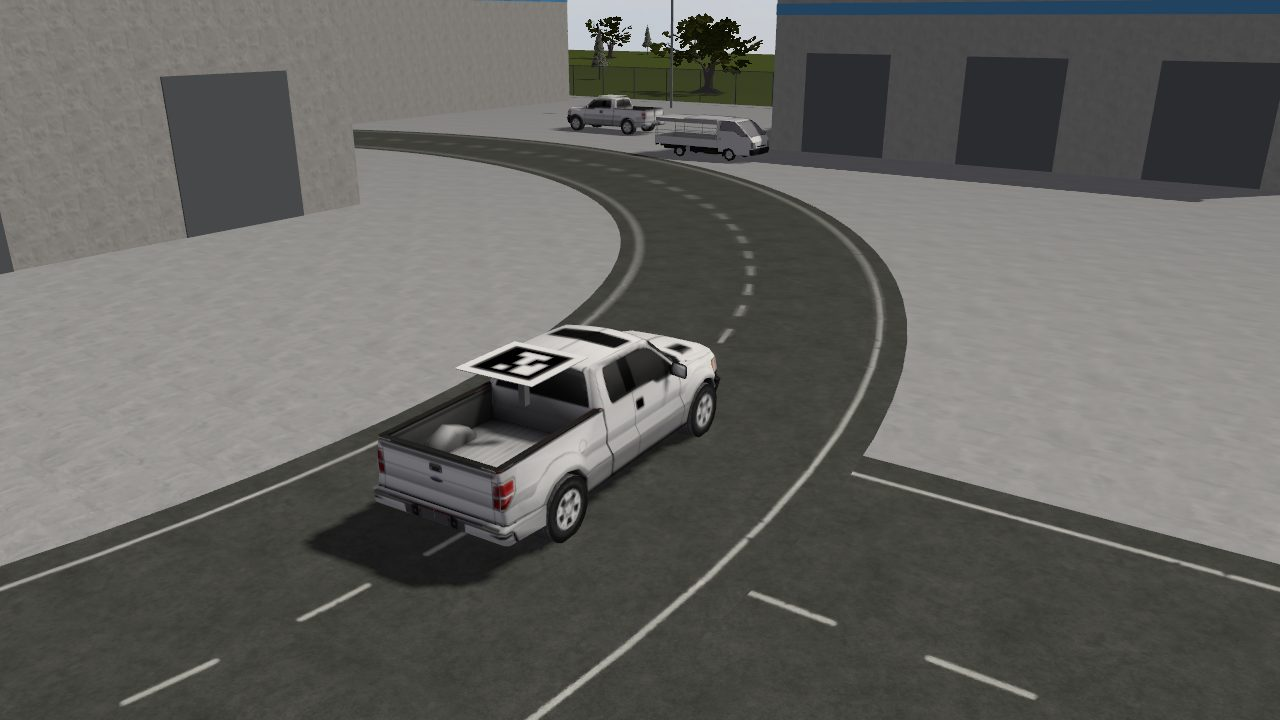
\includegraphics[width=\linewidth]{zona_bodegas_camioneta}
    \column{0.47\textwidth}\small
    \textbf{Escenario}: una camioneta sospechosa da vueltas en una zona de bodegas. Hay que
    \textbf{encontrarla}, \textbf{identificarla} por el ArUco 7 de su techo (no los señuelos),
    \textbf{dar su ubicación GPS} y \textbf{seguirla} desde arriba.
    \begin{itemize}
      \item Va a 3 m/s, una vuelta cada 55 s.
      \item \textbf{Lo nuevo}: perseguir algo que se \textbf{mueve}.
    \end{itemize}
  \end{columns}
\end{frame}

\begin{frame}{Buscar: el barrido ``podadora''}
  \begin{columns}[c]
    \column{0.47\textwidth}\centering
    \begin{tikzpicture}[x=0.045cm,y=0.045cm]
      \draw[gray!50,fill=gray!10] (-55,-12) rectangle (55,85);
      \draw[gray!60,line width=4pt,opacity=0.5] (0,42) circle (26.5);
      \draw[azul,thick,-{Stealth}] (-37.5,0) -- (-37.5,78) -- (-12.5,78) -- (-12.5,0) -- (12.5,0) -- (12.5,78) -- (37.5,78) -- (37.5,0);
      \draw[azul!30,line width=0.1pt,fill=azul!8,opacity=0.5] (-55,30) rectangle (-20,56);
      \node[font=\tiny,azul] at (-37.5,60) {ve};
      \node[draw,circle,fill=azulclaro,inner sep=0.5pt,font=\tiny] at (0,0) {H};
      \node[font=\tiny] at (0,42) {anillo};
    \end{tikzpicture}
    \column{0.5\textwidth}\small
    A 15 m, con 100° de campo, la cámara ve
    \[ 2\,h\tan(50°) \approx 36\ \text{m de ancho} \]
    Carriles norte--sur cada 25 m (se traslapan un poco) cubren todo el patio.
    \vspace{0.3em}

    Entre carriles avanza a \cmd{search\_speed} (5 m/s) con un punto que va 1 s adelante del dron y
    la velocidad como feedforward: si va muy rápido la cámara no alcanza a ver.
  \end{columns}
\end{frame}

\begin{frame}{Señuelos: filtrar por id}
  \begin{columns}[c]
    \column{0.45\textwidth}\centering
    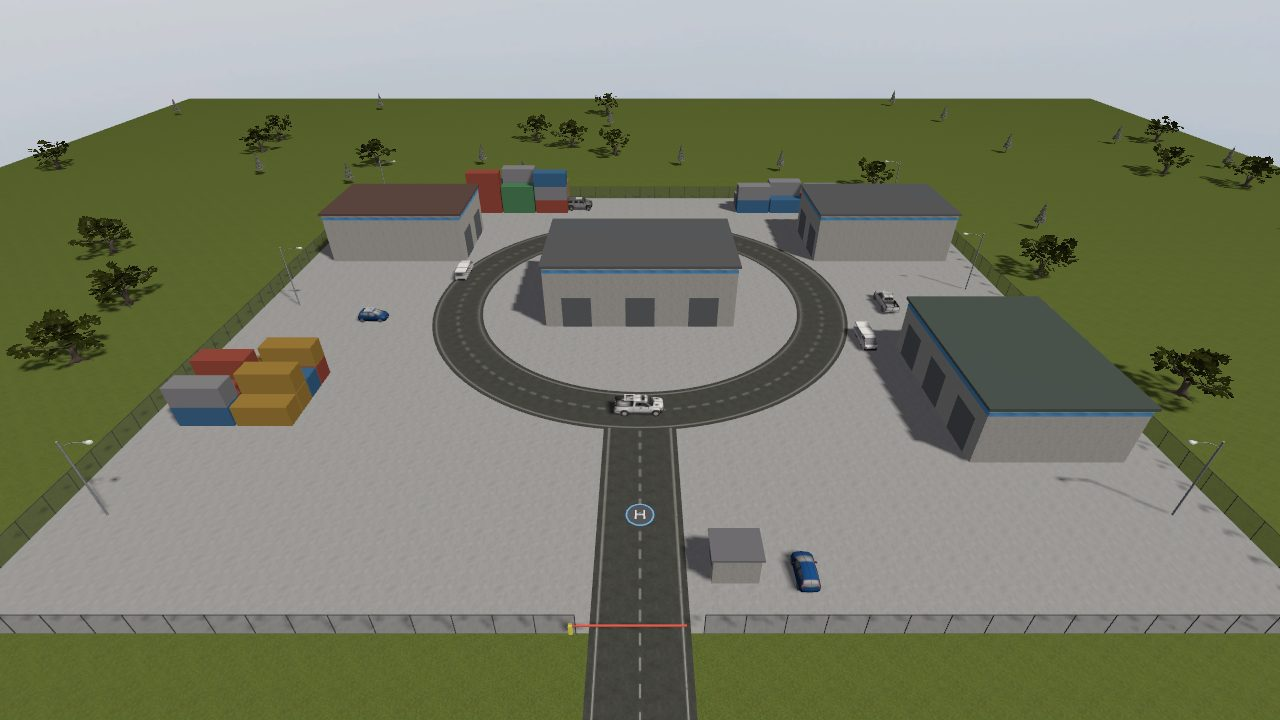
\includegraphics[width=0.9\linewidth]{zona_bodegas}
    \column{0.52\textwidth}\small
    Los coches estacionados también llevan ArUco (3, 12 y 25). El nodo los anuncia una vez y los ignora:
    \begin{terminal}{caza\_objetivo}
Veo el ArUco 3: es un señuelo, lo ignoro\\
Veo el ArUco 25: es un señuelo, lo ignoro\\
¡OBJETIVO ENCONTRADO! ArUco 7 en NED\\
\ norte 62.9, este 5.1 (lat ..., lon ...)
    \end{terminal}
  \end{columns}
\end{frame}

\begin{frame}{Seguir algo que se mueve}
  \begin{columns}[c]
    \column{0.47\textwidth}\centering
    \begin{tikzpicture}[scale=0.8]
      \draw[gray,thick] (0,0) -- (5,0);
      \fill[gray] (1.5,0) circle (3pt) node[below,font=\tiny] {donde se vio};
      \fill[naranja] (3.0,0) circle (3pt) node[below,font=\tiny] {donde está};
      \fill[verde] (3.7,0) circle (3pt) node[above,font=\tiny] {a donde ir};
      \draw[-{Stealth},thick,naranja] (3,0.3) -- (3.9,0.3) node[right,font=\tiny] {$v$};
      \draw[decorate,decoration={brace,amplitude=3pt}] (1.5,0.6) -- (3.7,0.6) node[midway,above=3pt,font=\tiny] {$v\,(\text{edad} + \text{adelanto})$};
    \end{tikzpicture}
    \column{0.5\textwidth}\small
    Si vas a donde la \emph{viste}, cuando llegas ya no está ahí. Hay que:
    \begin{enumerate}
      \item \textbf{Estimar su velocidad} (TODO 1).
      \item \textbf{Predecir} y mandar \textbf{feedforward} (TODO 2):
        \[ \mathbf{p}_{sp} = \mathbf{p}_{\text{vista}} + \mathbf{v}\,(\text{edad} + \text{lead}) \qquad
           \mathbf{v}_{sp} = \mathbf{v} \]
    \end{enumerate}
  \end{columns}
\end{frame}

\begin{frame}{TODO 1: estimar la velocidad}
  \small Con dos vistas de la camioneta, $(\mathbf{p}_1, t_1)$ y $(\mathbf{p}_2, t_2)$:
  \[ \mathbf{v}_{\text{cruda}} = \frac{\mathbf{p}_2 - \mathbf{p}_1}{t_2 - t_1} \]
  Cada vista trae ruido (píxeles, actitud): la velocidad cruda brinca. Se suaviza con un
  \textbf{filtro paso-bajas}:
  \[ \mathbf{v} \leftarrow \alpha\,\mathbf{v}_{\text{cruda}} + (1-\alpha)\,\mathbf{v}, \qquad \alpha \approx 0.3 \]
  \begin{columns}[c]
    \column{0.55\textwidth}
    \begin{itemize}
      \item Solo si la vista anterior es \textbf{reciente} (\textless 2 s).
      \item Y no \textbf{demasiado cercana} (\textgreater 0.25 s): con $\Delta t$ chico, el ruido domina.
    \end{itemize}
    \column{0.42\textwidth}
    \begin{tikzpicture}[x=0.5cm,y=0.6cm]
      \draw[-{Stealth}] (0,0) -- (7,0) node[right,font=\tiny] {t};
      \draw[gray] plot coordinates {(0,1.2) (0.5,2.2) (1,0.6) (1.5,2.0) (2,0.9) (2.5,1.9) (3,1.1) (3.5,1.7) (4,0.8) (4.5,1.6) (5,1.2) (5.5,1.5) (6,1.0)};
      \draw[verde,thick,smooth] plot coordinates {(0,0.4) (1,0.9) (2,1.1) (3,1.25) (4,1.28) (5,1.3) (6,1.3)};
      \node[font=\tiny,gray] at (1.4,2.5) {cruda};
      \node[font=\tiny,verde] at (5,0.6) {filtrada};
    \end{tikzpicture}
  \end{columns}
\end{frame}

\begin{frame}{Estados y calificación de la caza}
  \begin{columns}[c]
    \column{0.45\textwidth}
    \begin{tikzpicture}[node distance=0.3cm,st/.style={draw=azul,fill=azulclaro,rounded corners,font=\tiny,minimum width=1.6cm}]
      \node[st] (s) {SEARCH};
      \node[st,right=0.8cm of s,fill=yellow!20] (f) {FOLLOW};
      \node[st,below=0.7cm of f] (l) {LOST};
      \node[st,below=0.7cm of s] (r) {RETURN};
      \draw[-{Stealth}] (s) -- node[above,font=\tiny]{ve el 7} (f);
      \draw[-{Stealth}] (f) -- node[right,font=\tiny]{3 s sin verlo} (l);
      \draw[-{Stealth}] (l) to[bend right=30] node[right,font=\tiny,pos=0.3]{lo vuelve a ver} (f);
      \draw[-{Stealth}] (l) -- node[below,font=\tiny]{8 s} ++(-1.9,-0.0) |- (s);
      \draw[-{Stealth}] (f) to[bend right=45] node[above,font=\tiny,pos=0.6]{60 s} (r.north east);
    \end{tikzpicture}
    \column{0.52\textwidth}\small
    Durante los 60 s de seguimiento el nodo mide:
    \begin{itemize}
      \item \textbf{A la vista} $\geq$ 80\% del tiempo.
      \item \textbf{Distancia promedio} dron--camioneta (horizontal) $< 1.5$ m.
    \end{itemize}
    Sin los TODO, el dron va a donde la \emph{vio}, se queda atrás y el promedio no pasa.
  \end{columns}
\end{frame}

% ----------------------------------------------------------------------------- 7
\begin{frame}{Misión 7: la estación de carga}
  \begin{columns}[c]
    \column{0.5\textwidth}
    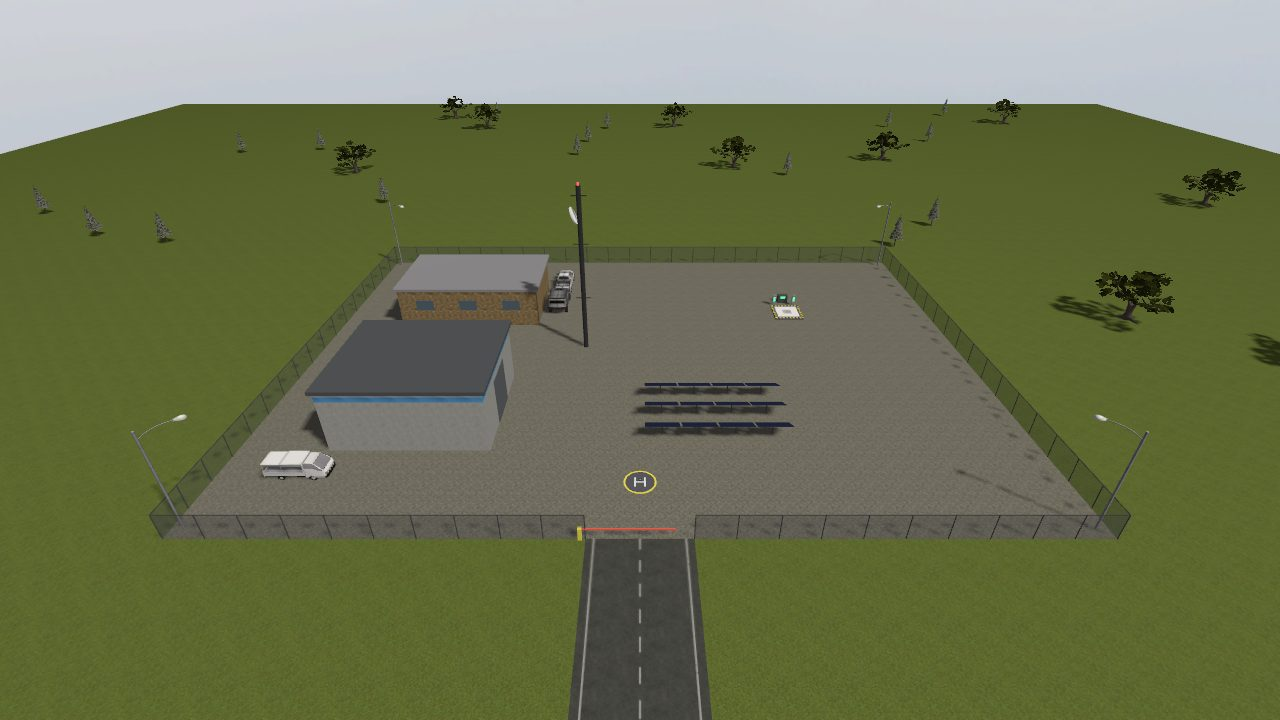
\includegraphics[width=\linewidth]{base_carga}
    \column{0.47\textwidth}\small
    \textbf{Escenario}: un dron de vigilancia patrulla la cerca de una base. Con batería baja, deja la
    patrulla, va a su estación, \textbf{aterriza con precisión} sobre el ArUco 42, ``carga'' y
    \textbf{regresa a patrullar justo donde se quedó}.
    \begin{itemize}
      \item \textbf{Viene de}: \cmd{battery\_monitor} + \cmd{square\_mission}.
    \end{itemize}
  \end{columns}
\end{frame}

\begin{frame}{La batería en PX4 SITL}
  \begin{columns}[c]
    \column{0.47\textwidth}
    \begin{tikzpicture}[x=0.11cm,y=0.025cm]
      \draw[-{Stealth}] (0,0) -- (62,0) node[right,font=\tiny] {s armado};
      \draw[-{Stealth}] (0,0) -- (0,110) node[above,font=\tiny] {\%};
      \draw[azul,thick] (0,100) -- (30,50) -- (40,50);
      \draw[verde,thick] (40,50) -- (40,100) -- (55,75);
      \draw[rojo,dashed] (0,60) -- (60,60) node[right,font=\tiny] {low\_percent};
      \node[font=\tiny,verde] at (40,106) {desarma = 100 \%};
      \node[font=\tiny,azul] at (18,40) {50 \% mínimo};
    \end{tikzpicture}
    \column{0.5\textwidth}\small
    \begin{itemize}
      \item Armado, baja de 100\% a 50\% en 30 s (\cmd{SIM\_BAT\_DRAIN} = 60 s) y \textbf{se queda en 50\%}.
      \item Al \textbf{desarmar} vuelve a 100\% al instante.
      \item O sea: aterrizar en la estación y desarmar \textbf{es cargar}.
      \item \cmd{low\_percent} tiene que ser $> 0.5$ (si no, nunca se dispara).
      \item Se lee de \cmd{/fmu/out/battery\_status\_v1} (\cmd{remaining}, 0--1, a 1 Hz).
    \end{itemize}
  \end{columns}
\end{frame}

\begin{frame}{La patrulla y la máquina de estados}
  \begin{columns}[c]
    \column{0.42\textwidth}\centering
    \begin{tikzpicture}[x=0.042cm,y=0.042cm]
      \draw[gray!50,fill=gray!10] (-35,-6) rectangle (35,46);
      \draw[azul,thick,-{Stealth}] (-31,-2) -- (-31,42) -- (31,42) -- (31,-2) -- (-31,-2);
      \fill[orange] (16.3,28.3) rectangle (19.7,31.7);
      \node[font=\tiny,right] at (20,30) {estación};
      \node[draw,circle,fill=azulclaro,inner sep=0.5pt,font=\tiny] at (0,0) {H};
      \fill[gray!60] (-27,4) rectangle (-13,16); \node[font=\tiny] at (-20,10) {hangar};
    \end{tikzpicture}
    \column{0.55\textwidth}
    \begin{tikzpicture}[node distance=0.22cm,st/.style={draw=azul,fill=azulclaro,rounded corners,font=\tiny,minimum width=1.9cm}]
      \node[st] (p) {PATROL};
      \node[st,right=0.4cm of p] (s) {TO\_STATION};
      \node[st,below=of s,fill=yellow!20] (pr) {PRECISION};
      \node[st,below=of pr] (la) {LANDING};
      \node[st,below=of la] (ch) {CHARGING};
      \node[st,left=0.4cm of ch] (re) {REARM / TAKEOFF};
      \node[st,above=of re] (rs) {RESUME};
      \draw[-{Stealth}] (p) -- node[above,font=\tiny]{batería} (s);
      \draw[-{Stealth}] (s) -- (pr); \draw[-{Stealth}] (pr) -- (la); \draw[-{Stealth}] (la) -- (ch);
      \draw[-{Stealth}] (ch) -- (re); \draw[-{Stealth}] (re) -- (rs); \draw[-{Stealth}] (rs) -- (p);
    \end{tikzpicture}
  \end{columns}
  \vspace{0.3em}
  \small Al dejar la patrulla guarda \textbf{dónde estaba y en qué tramo}; al volver, va ahí primero.
  Patrulla a 8 m y a 4 m de la cerca: lejos del hangar (6.5 m de alto) y la comandancia.
\end{frame}

\begin{frame}{El GPS te lleva cerca; la cámara te pone encima}
  \begin{columns}[c]
    \column{0.47\textwidth}\centering
    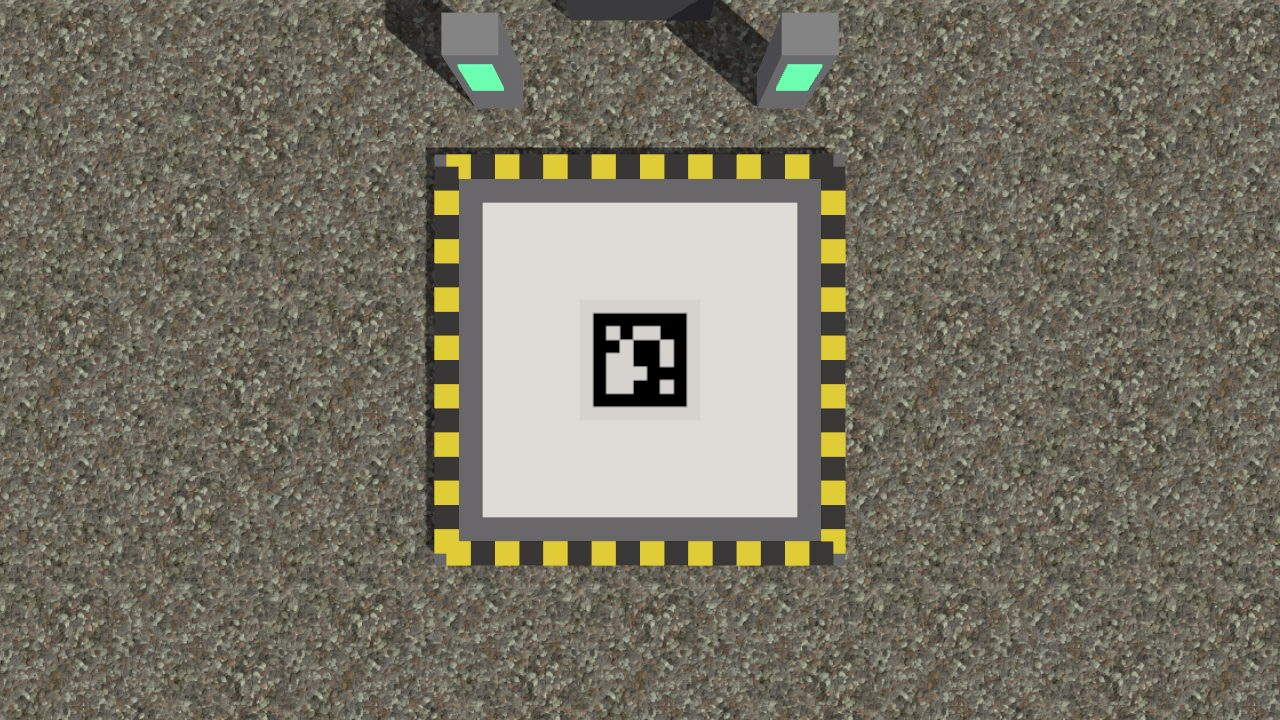
\includegraphics[width=0.9\linewidth]{base_carga_estacion}
    \column{0.5\textwidth}\small
    La estación ``según el mapa'' (\cmd{station\_north/east}) tiene \textbf{1.5 m de error a propósito}:
    la plataforma real está en N 30, E 18.
    \vspace{0.3em}

    \textbf{TODO}: en cada ciclo de la bajada, un setpoint mixto:
    \begin{itemize}
      \item en $x, y$: \textbf{posición} = donde ve el ArUco;
      \item en $z$: \textbf{velocidad} = bajar a \cmd{descent\_speed} solo si ya está \textbf{centrado}
        (\textless 0.2 m); si no, 0 mientras se acomoda;
      \item si no lo ve: quieto y subir un poco para que vuelva a caber en la imagen.
    \end{itemize}
  \end{columns}
\end{frame}

\begin{frame}{Bajar centrado}
  \begin{columns}[c]
    \column{0.45\textwidth}\centering
    \begin{tikzpicture}[scale=0.8]
      \fill[gray!40] (-1.7,0) rectangle (1.7,0.25);
      \fill[black] (-0.35,0.25) rectangle (0.35,0.3);
      \draw[azul,thick,-{Stealth}] (1.5,4) -- (0.3,3.4);
      \draw[azul,thick,-{Stealth}] (0.3,3.4) -- (0,3.1);
      \draw[verde,thick,-{Stealth}] (0,3.1) -- (0,0.9);
      \node[font=\tiny,right] at (1.5,4) {llega por GPS (1.5 m chueco)};
      \node[font=\tiny,right] at (0.35,3.25) {se centra sin bajar};
      \node[font=\tiny,right] at (0.1,2) {baja centrado};
      \draw[rojo,dashed] (-1.8,0.8+0.25) -- (1.8,0.8+0.25) node[right,font=\tiny] {0.8 m: Land};
    \end{tikzpicture}
    \column{0.52\textwidth}\small
    \begin{itemize}
      \item A \textasciitilde0.8 m sobre la plataforma, PX4 termina con \cmd{land()}: detecta el contacto y
        desarma.
      \item \textbf{Éxito}: cada carga aterriza a \textbf{menos de 0.3 m} del centro del ArUco.
      \item Sin el TODO baja derecho sobre la coordenada del mapa y aterriza \textasciitilde1.5 m chueco.
    \end{itemize}
    \begin{terminal}{al terminar}
carga 1: aterrizó a ... m del centro\\
\ \ (máximo 0.3) OK / FALLÓ
    \end{terminal}
  \end{columns}
\end{frame}

% =============================================================================
\section{Calificar, depurar y chuleta}
% =============================================================================

\begin{frame}{Criterio de éxito de cada misión}
  \centering\scriptsize
  \begin{tabular}{clp{8.2cm}}
    \toprule
    \# & Misión & El nodo imprime ``Misión cumplida'' si\ldots \\
    \midrule
    1 & Estrella & pasa a \textless 0.5 m de cada vértice, regresa al centro y aterriza \\
    2 & Pilar & radio $3 \pm 0.3$ m, yaw \textless 10°, $\geq$ 90\% de las vueltas y llega a 4 m \\
    3 & Entrega & secuencia completa sin tocar QGC y termina a \textless 1.5 m de la H de la farmacia \\
    4 & Geocerca & el dron se detiene antes de pasar 1 m la cerca (prueben 2 y 6 m/s, varias direcciones) \\
    5 & Cueva & cruza, el lidar nunca a \textless 0.6 m de la roca, aterriza a \textless 1 m de la plataforma \\
    6 & Caza & a la vista $\geq$ 80\% de 60 s y a \textless 1.5 m en promedio \\
    7 & Estación & cada carga aterriza a \textless 0.3 m del centro del ArUco y termina la patrulla \\
    \bottomrule
  \end{tabular}
\end{frame}

\begin{frame}{La rúbrica}
  \centering\small
  \begin{tabular}{lrp{7cm}}
    \toprule
    Criterio & Peso & Qué se revisa \\
    \midrule
    Funciona & 40\% & ``Misión cumplida'' en 3 corridas seguidas \\
    Manejo de fallas & 15\% & Aborta y regresa bien cuando se le provoca una falla \\
    Código legible & 20\% & Máquina de estados clara, comentarios como en \cmd{px4\_examples} \\
    Parámetros & 10\% & Se ajusta con \cmd{--ros-args} sin recompilar \\
    README + video & 15\% & Otra persona lo corre solo con el README \\
    \bottomrule
  \end{tabular}
  \vspace{0.6em}
  \begin{idea}
    \small Cada quien presenta su misión en 5 minutos frente al equipo. Explicar la máquina de estados en voz
    alta es donde se nota si de verdad la entendieron.
  \end{idea}
\end{frame}

\begin{frame}{Provocar fallas a propósito}
  \small El 15\% de ``manejo de fallas'' se prueba así:
  \begin{itemize}
    \item \textbf{Matar el nodo} a media misión (Ctrl+C): en offboard PX4 debe entrar en failsafe;
      con comandos (misión 3) se queda en Hold.
    \item \textbf{Tomar el control desde QGC} (cambiar a Position o Hold): el nodo debe soltar y avisar
      ``Fuera de OFFBOARD''.
    \item \textbf{Geocerca}: escaparse en distintas direcciones y velocidades con \cmd{vuelo\_prueba}.
    \item \textbf{Cueva}: subir \cmd{max\_speed} o bajar \cmd{stop\_distance} hasta que falle; ¿cómo falla?
    \item \textbf{Estación}: subir \cmd{low\_percent} a 0.9 para que vaya a cargar más seguido.
  \end{itemize}
\end{frame}

\begin{frame}{Problemas comunes (1/2)}
  \centering\scriptsize
  \begin{tabular}{p{4.4cm}p{8.4cm}}
    \toprule
    Síntoma & Causa y arreglo \\
    \midrule
    No arma; \cmd{No connection to the GCS} & QGC no está abierto: \cmd{vespo qgc} (o usar \cmd{vespo up --sim}) \\
    \cmd{PX4 rechazó el comando 176} & El modo pedido no se puede ahora (p. ej. armar desde Land): pasar por Hold \\
    El dron se va al suelo o hacia arriba & Signo de $z$: en NED arriba es negativo \\
    La trayectoria se adelanta al dron & Tiempo con \cmd{now()} y la simulación lenta: usar \cmd{px4\_.clock()} \\
    ``Fuera de OFFBOARD'' sin tocar nada & El nodo dejó de publicar \textgreater0.5 s (un \cmd{return} antes de \cmd{offboard()}, un bloqueo) \\
    \bottomrule
  \end{tabular}
\end{frame}

\begin{frame}{Problemas comunes (2/2)}
  \centering\scriptsize
  \begin{tabular}{p{4.4cm}p{8.4cm}}
    \toprule
    Síntoma & Causa y arreglo \\
    \midrule
    \cmd{/x500/scan} o \cmd{/x500/camera/image} vacíos & El puente no está: usar el \emph{launch}; revisar el modelo (\cmd{--custom}) y el nombre del mundo \\
    El detector no ve nada & Falta \cmd{camera\_info} (el detector la espera), marcador muy chico o sin margen blanco \\
    La RAM de Gazebo crece sin parar & Cámara pesada o plugin de video de PX4: usar \cmd{x500\_cam\_abajo} y nuestros mundos \\
    La laptop se apaga sola & Sin cargador: conectar \\
    Un mundo modificado no cambia & Faltó \cmd{build\_worlds.py} y \cmd{vespo build} \\
    \bottomrule
  \end{tabular}
\end{frame}

\begin{frame}[fragile]{Chuleta}
  \begin{lstlisting}[style=bash,caption={Lo de todos los días}]
vespo build                                            # compilar
vespo up --sim --world <mundo> [--custom <modelo>]      # simular
ros2 run x500_retos <nodo> --ros-args -p <param>:=<valor>
ros2 launch x500_retos {cueva,caza,estacion}.launch.py
ros2 topic echo /fmu/out/vehicle_status_v1 --field nav_state
ros2 run rqt_image_view rqt_image_view /x500/aruco/debug
python3 src/x500_retos/tools/build_worlds.py            # regenerar mundos
gz topic -e -t /world/<mundo>/stats -n 1 | grep real_time   # ¿va a 1.0x?
  \end{lstlisting}
\end{frame}

\begin{frame}{Para cerrar}
  \begin{columns}[c]
    \column{0.55\textwidth}\small
    \begin{enumerate}
      \item \textbf{Nivel 1}: muévanse bien (geometría, derivadas, comandos).
      \item \textbf{Nivel 2}: que el dron decida (predecir, reaccionar a un sensor).
      \item \textbf{Nivel 3}: que vea (percepción separada del control).
    \end{enumerate}
    \vspace{0.4em}
    No se salta de nivel sin cerrar al menos dos misiones del anterior.
    \column{0.42\textwidth}\centering
    
\includegraphics[width=0.75\linewidth]{vespo_logo}\\[0.5em]
    {\Large ¿Preguntas?}
  \end{columns}
\end{frame}


\end{document}
